\PassOptionsToClass{}{beamer}
\documentclass[serif, aspectratio=169]{beamer}
\usepackage[utf8]{inputenc}
\usepackage{amsmath,esint}
\usepackage[british]{babel}
\usetheme{Warsaw}
\usecolortheme{rose}
\usepackage{comment}
\usepackage{pgfplots}
\usepackage{ mathrsfs }
\usepackage{gensymb}
\usepackage{color}
\usepackage{tkz-euclide}
\usetkzobj{all}
\usepackage{tkz-fct}  
\usetikzlibrary{calc}
\usepackage[ruled]{algorithm2e}
\usepackage{tikz}
\usepackage{animate}
\usepackage{ragged2e}
\usepackage{mwe}
\DeclareMathOperator*{\minimize}{minimize}

\addtobeamertemplate{navigation symbols}{}{%
    \usebeamerfont{footline}%
    \usebeamercolor[fg]{footline}%
    \hspace{1em}%
    \insertframenumber/\inserttotalframenumber
}

\makeatletter
\newcommand\titlegraphicii[1]{\def\inserttitlegraphicii{#1}}
\titlegraphicii{}
\setbeamertemplate{title page}
{
  \vspace{0.3in}
  \vbox{}

  \begin{centering}
    \begin{beamercolorbox}[sep=8pt,center]{title}
      \usebeamerfont{title}\inserttitle\par%
      \ifx\insertsubtitle\@empty%
      \else%
        \vskip0.25em%
        {\usebeamerfont{subtitle}\usebeamercolor[fg]{subtitle}\insertsubtitle\par}%
      \fi%     
    \end{beamercolorbox}%
    \vskip1em\par
    \begin{beamercolorbox}[sep=8pt,center]{date}
      \usebeamerfont{date}\insertdate
    \end{beamercolorbox}%\vskip0.5em
    \begin{beamercolorbox}[sep=8pt,center]{author}
      \usebeamerfont{author}\insertauthor
    \end{beamercolorbox}
    \begin{beamercolorbox}[sep=8pt,center]{institute}
      \usebeamerfont{institute}\insertinstitute
    \end{beamercolorbox}
  \end{centering}
  %\vfill
}
\makeatother

\author{Mitesh M. Khapra}
\title{CS7015 (Deep Learning) : Lecture 5}
\subtitle{Gradient Descent (GD), Momentum Based GD, Nesterov Accelerated GD, Stochastic GD, AdaGrad, RMSProp, Adam}
\institute{Department of Computer Science and Engineering\\ Indian Institute of Technology Madras}
\date{February 2, 2018}
\titlegraphic{
\includegraphics[height=1cm,width=2cm]{images/iitm_logo.png}}


\begin{document}



\def\alpha{8} 

\newcommand\myheading[1]{%
\par\bigskip
{\Large\bfseries#1}\par\smallskip}


\newcommand\derivative[5]{%
    \tkzDefPointByFct[draw](#1) \tkzGetPoint{start}
  \tkzDefPointByFct[draw](#2) \tkzGetPoint{end}
  \draw[thin,|-|,yshift=-3pt] (start) -- node[black,fill=white,#5] {#3}(start-|end);  
  \draw[thin,|-|,xshift=3pt] (start-|end) -- node[black,fill=white,right] {#4}(end); 
  %\draw[thin] (start) --(end); 
}

\maketitle

\begin{frame}
	\begin{block}{Acknowledgements}
		\begin{itemize}\justifying
			%\footnote{xx}
			\item For most of the lecture, I have borrowed ideas from the videos by Ryan Harris on ``visualize backpropagation'' (available on youtube)
			\item Some content is based on the course CS231n\footnote{http://cs231n.stanford.edu/2016/} by Andrej Karpathy and others
		\end{itemize}
	\end{block}
\end{frame}

\begin{frame}
	\myheading{Module 5.1: Learning Parameters : Infeasible (Guess Work)}
\end{frame}

\begin{frame}
	
	\begin{columns}
		
		\column{0.5\textwidth}
		\begin{overlayarea}{\textwidth}{\textheight}
			
\begin{tikzpicture}
	\node (input2) at (10,-0.1)  {$x_{1}$};
	\node [hidden_neuron] (neuron1) at (10,2)  {};
	\node (output0)  at (10,3.5) {$y$};
	\draw [->] (input2) -- (neuron1);
	\draw [->] (neuron1) -- (output0);
	\node (bias) at (8, 2) {$bias = w_0 = -0.5$};
	\node (weight) at (9.4,0.6) {$w_1 = 1$};
	\onslide<3->{\node (text) at (10,-0.7) {$criticsRating$};}
\end{tikzpicture}
			\only<4->{
				\vspace{-0.2in}
				\begin{figure}[!htp]
					\begin{center}
						\includegraphics<4-7>[scale=0.3]{images/module1/2sample_points.png}
						\includegraphics<8->[scale=0.3]{images/module1/2sample_points_sigmoid.png}
					\end{center}
				\end{figure}
			}
		\end{overlayarea}
		
		\column{0.5\textwidth}<2->
		\begin{overlayarea}{\textwidth}{\textheight}
			\only<2-3>{
				\begin{block}<2-3>{Input for training}
					$\{x_i, y_i\}^{N}_{i=1} \rightarrow N$ pairs of $(x,y)$
				\end{block}
				\begin{block}<3>{Training objective}
					Find $w$ and $b$ such that:\\
					$\displaystyle{\minimize_{w,b} \mathscr{L}(w,b) = \sum_{i=1}^{N} (y_i - f(x_i))^2}$
				\end{block}
			}
			
			\only<4->{
				\begin{block}{What does it mean to train the network?}
					\begin{itemize}\justifying
						\item<4-> Suppose we train the network with $ (x, y) = (0.5, 0.2)$ and $(2.5, 0.9)$  
						\item<5-> At the end of training we expect to find $w^*$, $b^*$ such that:
						\item<6-> $f(0.5) \rightarrow 0.2$ and  $f(2.5) \rightarrow 0.9$
					\end{itemize}
					
				\end{block}
				
				\begin{block}<7->{In other words...}
					\begin{itemize}\justifying
						\item We hope to find a sigmoid function such that $(0.5, 0.2)$ and $(2.5, 0.9)$ lie on this sigmoid
					\end{itemize}
				\end{block}
				
			}
		\end{overlayarea}
	\end{columns}
\end{frame}

%\subsection{Curve-fitting}
\begin{frame}
	\fontsize{16pt}{7.2}\selectfont
	\textit{Let us see this in more detail....}
\end{frame}

\begin{frame}
	\begin{columns}
		\column{0.35\textwidth}
		\begin{overlayarea}{\textwidth}{\textheight}
			\begin{onlyenv}<1->
				\begin{figure}[!htp]
					\begin{center}
						\includegraphics<1-2>[scale=0.3]{images/module1/2sample_points.png}
						\includegraphics<3-11>[scale=0.3]{images/module1/random/sig0.png}
						\includegraphics<12>[scale=0.3]{images/module1/random/sig1.png}
						\includegraphics<13>[scale=0.3]{images/module1/random/sig2.png}
						\includegraphics<14>[scale=0.3]{images/module1/random/sig3.png}
						\includegraphics<15>[scale=0.3]{images/module1/random/sig4.png}
						\includegraphics<16->[scale=0.3]{images/module1/random/sig5.png}
					\end{center}
				\end{figure}  
			\end{onlyenv}
		\end{overlayarea}
		
		\column{0.65\textwidth}
		\begin{overlayarea}{\textwidth}{\textheight}
			\only<2-5>{
				\begin{itemize}\justifying
					\item Can we try to find such a $w^*, b^*$ manually
					      \item<3-> Let us try a random guess.. (say, $w=0.5, b=0$)
					      \item<4-> Clearly not good, but how bad is it ?
					      \item<5-> Let us revisit $\mathscr{L}(w,b)$ to see how bad it is ... 
				\end{itemize}
			}
			
			\only<6-10>{
				\begin{align*}
					\onslide<6->{\mathscr{L}(w,b) & = \frac{1}{2} * \sum_{i=1}^{N} (y_i - f(x_i))^2}     \\
					\onslide<7->{                 & = \frac{1}{2} * ((y_1 - f(x_1))^2 + (y_2 - f(x_2))^2)} \\
					\onslide<8->{                 & = \frac{1}{2} * ((0.9 - f(2.5))^2 + (0.2 - f(0.5))^2)} \\
					\onslide<9->{                 & = 0.073}                                             
				\end{align*}
				\only<10->{\parbox[c][50pt][c]{230pt}{We want $\mathscr{L}(w,b)$ to be as close to 0 as possible}}
			}
			
			\only<11-> {
				Let us try some other values of $w$, $b$ 
				
				\begin{flushleft}
					\begin{table}
						\begin{tabular}{ccc}
							\hline
							\hline
							$w$               & $b$   & $\mathscr{L}(w,b)$ \\
							\hline
							\hline
							0.50              & 0.00  & 0.0730             \\
							\onslide<12-> {-0.10 & 0.00  & 0.1481}            \\
							\onslide<13-> {0.94  & -0.94 & 0.0214}            \\
							\onslide<14-> {1.42  & -1.73 & 0.0028}            \\
							\onslide<15-> {1.65  & -2.08 & 0.0003}            \\
							\onslide<16-> {1.78  & -2.27 & 0.0000}            \\
							\hline
							\hline
						\end{tabular}
					\end{table}
				\end{flushleft}
				
				\only<12>{\parbox[c][50pt][c]{230pt}{Oops!! this made things even worse...}}
				\only<13>{\parbox[c][50pt][c]{230pt}{Perhaps it would help to push w and b in the other direction...}}
				\only<14-15>{\parbox[c][50pt][c]{230pt}{Let us keep going in this direction, \textit{i.e.}, increase $w$ and decrease $b$}}
				\only<16>{\parbox[c][50pt][c]{230pt}{With some guess work and intuition we were able to find the right values for $w$ and $b$}}
			}
		\end{overlayarea}
	\end{columns}
	
\end{frame}

%\subsection{Error surfaces}
\begin{frame}
	\fontsize{16pt}{7.2}\selectfont
	\textit{Let us look at something better than our ``guess work'' algorithm....}
\end{frame}

\begin{frame}
	\begin{columns}
		\column{0.5\textwidth}
		\begin{overlayarea}{\textwidth}{\textheight}
			\begin{onlyenv}<1->
				\begin{figure}[!htp]
					\begin{center}
						\includegraphics<2->[scale=0.5]{images/module1/error_surface1.png}
					\end{center}
				\end{figure}  
			\end{onlyenv}
		\end{overlayarea}
		
		\column{0.5\textwidth}
		\begin{overlayarea}{\textwidth}{\textheight}
			\begin{itemize}\justifying
				\item Since we have only 2 points and 2 parameters ($w$, $b$) we can easily plot $\mathscr{L}(w,b)$ for different values of ($w$, $b$) and pick the one where $\mathscr{L}(w,b)$ is minimum
				      \item<3-> But of course this becomes intractable once you have many more data points and many more parameters !!
				      \item<4-> Further, even here we have plotted the error surface only for a small range of ($w$, $b$) [from $(-6, 6)$ and not from $(-\inf, \inf)$]
			\end{itemize}
		\end{overlayarea}
	\end{columns}
\end{frame}

\begin{frame}
	\fontsize{16pt}{7.2}\selectfont
	\textit{Let us look at the geometric interpretation of our ``guess work'' algorithm in terms of this error surface}
\end{frame}


\begin{frame}
	\begin{columns}
		\column{0.5\textwidth}
		\begin{overlayarea}{\textwidth}{\textheight}
			\begin{figure}[!htp]
				\begin{center}
					\only<1>{\includegraphics[width=1.0\textwidth]{images/module1/2sample_points.png}}
					\only<2>{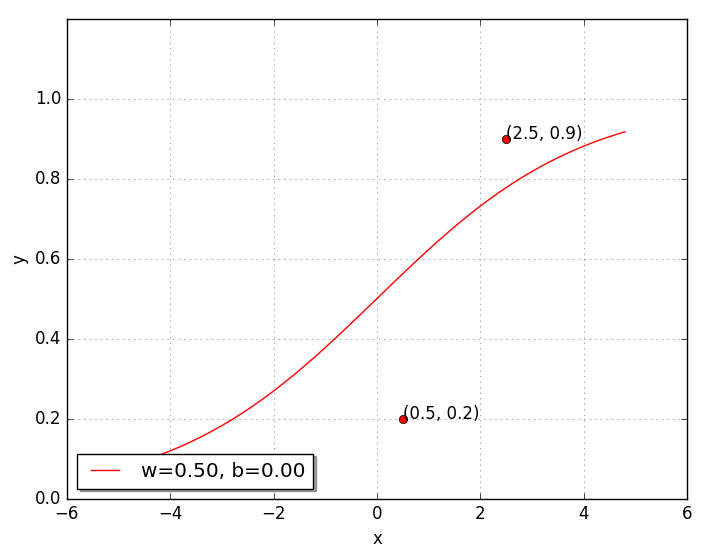
\includegraphics[width=1.0\textwidth]{images/module1/random/sig0.png}}
					\only<3>{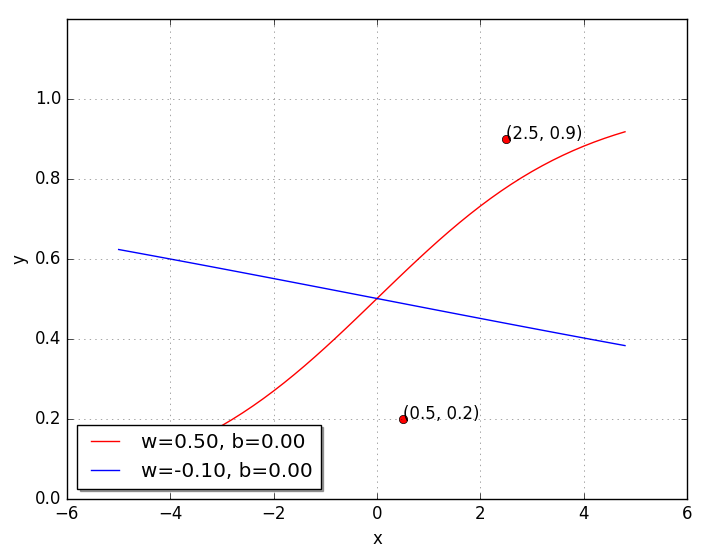
\includegraphics[width=1.0\textwidth]{images/module1/random/sig1.png}}
					\only<4>{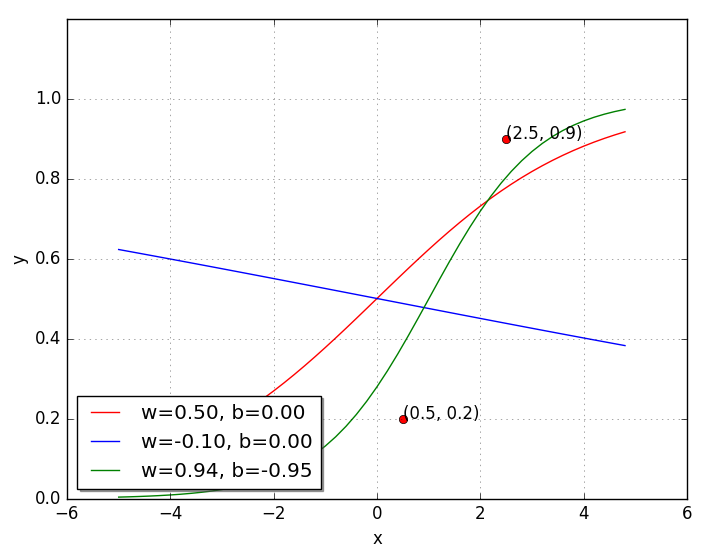
\includegraphics[width=1.0\textwidth]{images/module1/random/sig2.png}}
					\only<5>{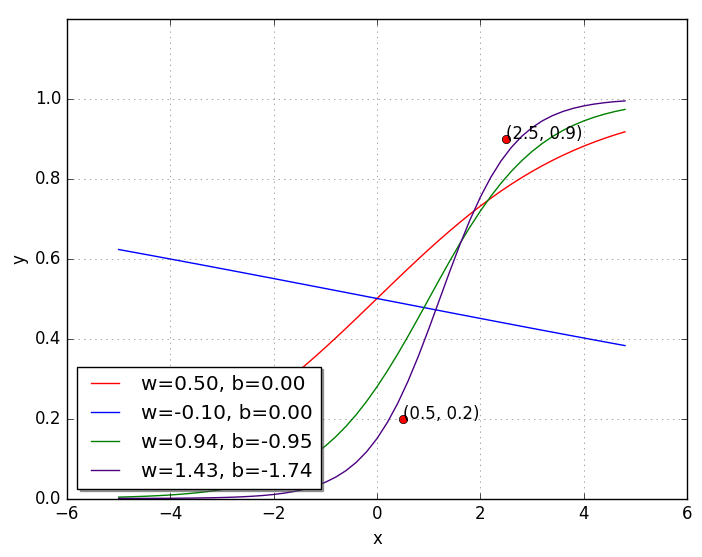
\includegraphics[width=1.0\textwidth]{images/module1/random/sig3.png}}
					\only<6>{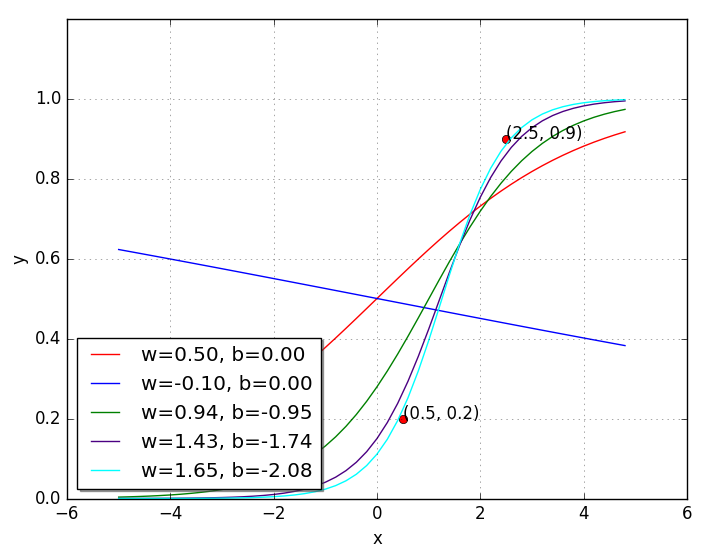
\includegraphics[width=1.0\textwidth]{images/module1/random/sig4.png}}
					\only<7->{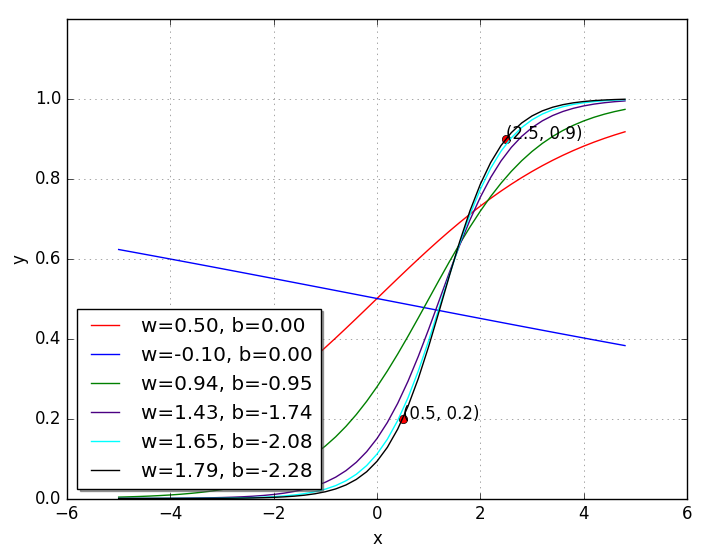
\includegraphics[width=1.0\textwidth]{images/module1/random/sig5.png}}
				\end{center}
			\end{figure}  
		\end{overlayarea}
		
		\column{0.5\textwidth}
		\begin{overlayarea}{\textwidth}{\textheight}
			\begin{figure}[!htp]
				\begin{center}
					\only<1>{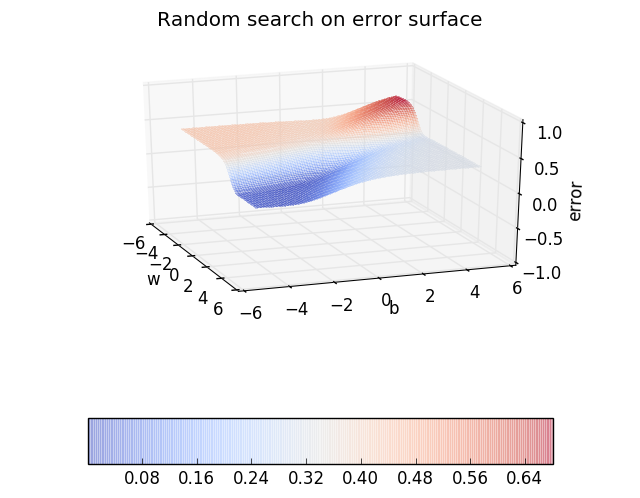
\includegraphics[width=1.0\linewidth]{images/module1/error_surface1.png}}
					\only<2>{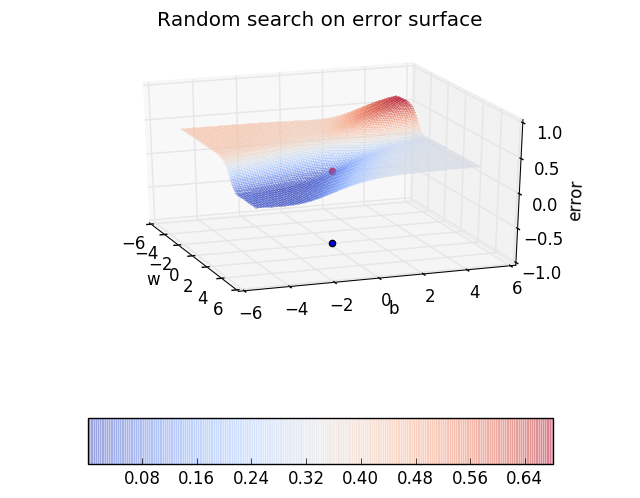
\includegraphics[width=1.0\linewidth]{images/module1/random/error0.png}}
					\only<3>{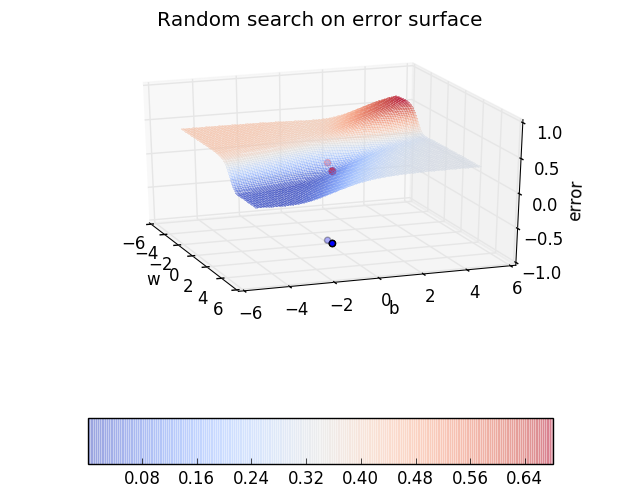
\includegraphics[width=1.0\linewidth]{images/module1/random/error1.png}}
					\only<4>{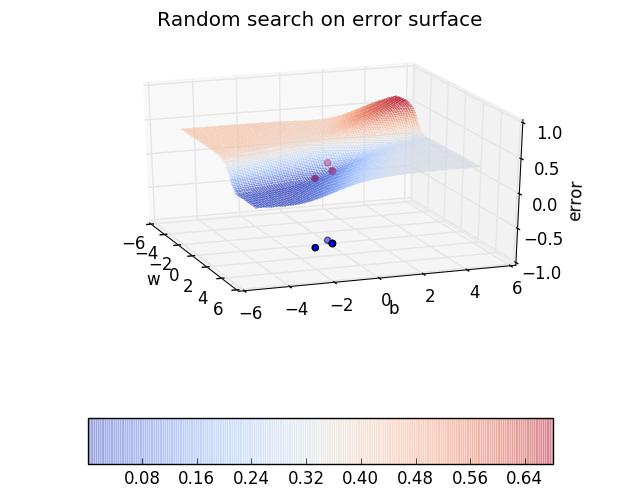
\includegraphics[width=1.0\linewidth]{images/module1/random/error2.png}}
					\only<5>{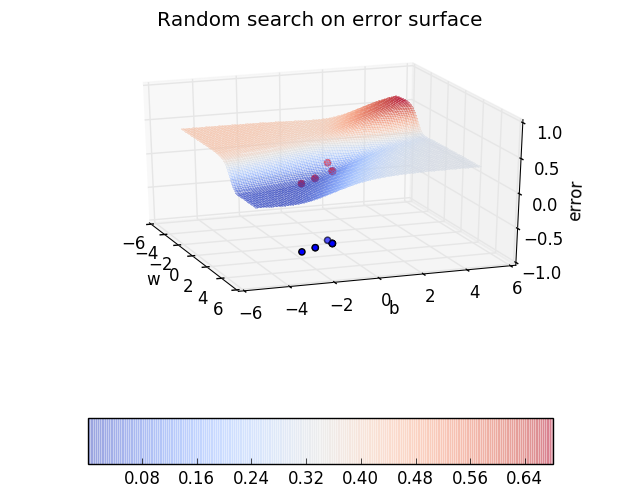
\includegraphics[width=1.0\linewidth]{images/module1/random/error3.png}}
					\only<6>{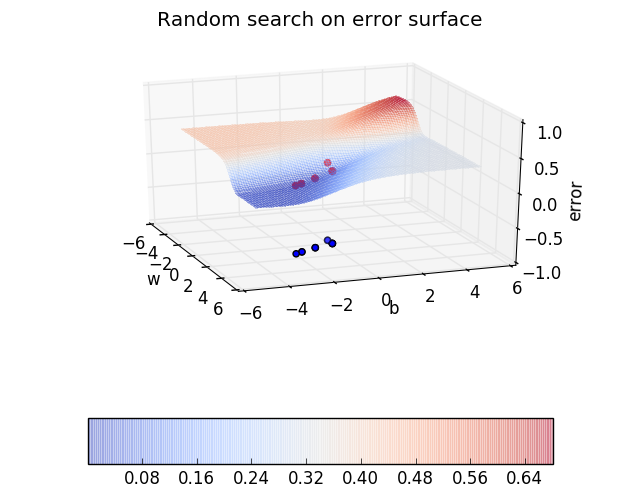
\includegraphics[width=1.0\linewidth]{images/module1/random/error4.png}}
					\only<7->{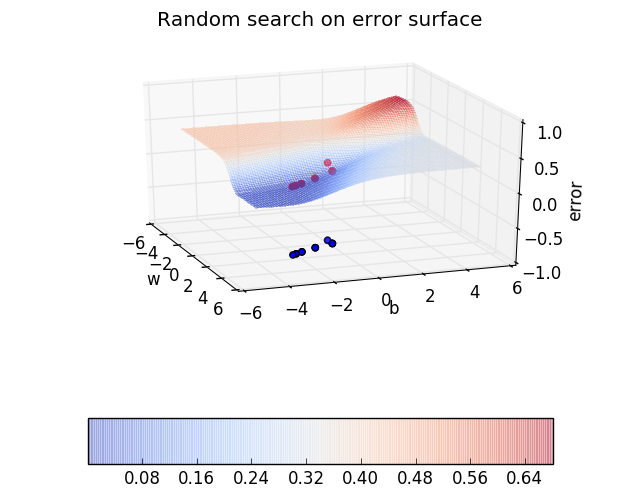
\includegraphics[width=1.0\linewidth]{images/module1/random/error5.png}}
				\end{center}
			\end{figure}  
		\end{overlayarea}
		
	\end{columns}
	
\end{frame}


\begin{frame}
	\myheading{Module 5.2: Learning Parameters : Gradient Descent}
\end{frame}

\begin{frame}
	\fontsize{16pt}{7.2}\selectfont
	\textit{Now let's see if there is a more efficient and principled way of doing this}
\end{frame}

%\section{Optimization methods}
%\subsection{Gradient Descent}
%\subsection{Goal}
\begin{frame}
	\begin{block}{Goal}
		Find a better way of traversing the error surface so that we can reach the minimum value quickly without resorting to brute force search! 
	\end{block}
\end{frame}


\begin{frame}
	\begin{overlayarea}{\textwidth}{\textheight}
		\begin{tikzpicture}
\begin{axis}[axis lines=left, ticks=none,xmax=0.5,ymax=0.5,x label style={at={(axis description cs:0.5,0)},anchor=north},
xlabel={$\theta$}, ylabel={error}]
\addplot[thick,black, no markers, samples=200, domain=-5:0] {-x*exp(x)};
\only<2->{\draw[dashed] (axis cs:-1.88,0.31) -- (axis cs:-0.0,0.31)} ;
\only<2->{\draw[dashed] (axis cs:-2.68,0.21) -- (axis cs:-0.0,0.21)} ;

\end{axis}
\end{tikzpicture}

	\end{overlayarea}
	
\end{frame}

%\subsection{Taylor series}
\begin{frame}
	\begin{overlayarea}{\textwidth}{\textheight}
		For ease of notation, let $\Delta\theta = u$, then from Taylor series, we have,
		
		\begin{align*}
			\only<2->{\mathscr{L}(\theta + \eta u) & =  \mathscr{L}(\theta)+ \eta*u^T \nabla\mathscr{L}(\theta) + \frac{\eta^2}{2!}*u^T \nabla^2\mathscr{L}(\theta)u + \frac{\eta^3}{3!}*... + \frac{\eta^4}{4!}*...} \\
			\only<3->{                             & = \mathscr{L}(\theta)+ \eta*u^T \nabla\mathscr{L}(\theta) \text{  } [\textit{$\eta$ is typically small, so $\eta^2, \eta^3,...\rightarrow 0$}]}                  
		\end{align*}
		
		\only<4->{Note that the move ($\eta u$) would be favorable only if,}
		\begin{align*}
			\only<4->{ & \mathscr{L}(\theta + \eta u) - \mathscr{L}(\theta) < 0 \textit{ }[\textit{i.e., if the new loss is less than the previous loss}]} \\
			\only<5->{\intertext {This implies,}}
			\only<5->{ & u^T \nabla\mathscr{L}(\theta) < 0}                                                                                      
		\end{align*}
	\end{overlayarea}
\end{frame}

\begin{frame}
	
	\begin{overlayarea}{\textwidth}{\textheight}
		Okay, so we have,
		\begin{align*}
			u^T \nabla\mathscr{L}(\theta) < 0 
		\end{align*}
		
		\only<1->{But, what is the range of $u^T \nabla\mathscr{L}(\theta)$ ?} \only<2->{Let's see....}\\
		
		\only<3->{Let $\beta$ be the angle between $u^T$ and $\nabla\mathscr{L}(\theta)$, then we know that,} 
		\only<4->{
			\begin{align*}
				\onslide<4->{-1 & \leq cos(\beta) = \frac{u^T \nabla\mathscr{L}(\theta)}{||u||*||\nabla\mathscr{L}(\theta)||} \leq 1} 
				%\only<5->{\intertext{Let's assume $u$ and $\mathscr{L}'(\theta)$ are unit vectors}}
				\onslide<5->{\intertext{Multiply throughout by $k = ||u||*||\nabla\mathscr{L}(\theta)||$ }}
				\onslide<5->{-k & \leq k*cos(\beta) = u^T \nabla\mathscr{L}(\theta) \leq k }                                          
				\onslide<6->{\intertext{Thus, $\mathscr{L}(\theta + \eta u) - \mathscr{L}(\theta) = u^T \nabla\mathscr{L}(\theta) = k*cos(\beta)$ will be most negative when $cos(\beta) =-1$ \textit{i.e.}, when $\beta$ is $180\degree$}}
			\end{align*}
		}
		
	\end{overlayarea}
\end{frame}

%\subsection{The update rule}
\begin{frame}
	\begin{overlayarea}{\textwidth}{\textheight}
		
		\begin{block}{Gradient Descent Rule}
			\begin{itemize}\justifying
				\item<1-> The direction $u$ that we intend to move in should be at $180\degree$ w.r.t. the gradient
				\item<2-> In other words, move in a direction opposite to the gradient
			\end{itemize}
		\end{block}
		
		\only<3->{
			\begin{block}{Parameter Update Equations}
				\vspace{-0.1in}
				\begin{align*}
					w_{t+1}             & = w_{t} - \eta \nabla w_{t}                                                 \\
					b_{t+1}             & = b_{t} - \eta \nabla b_{t}                                                 \\
					where, \nabla w_{t} & = \frac{\partial\mathscr{L}(w,b)}{\partial w}_{\textit{at $w=w_t, b=b_t$}}, 
					\nabla b_t = \frac{\partial\mathscr{L}(w,b)}{\partial b}_{\textit{at $w=w_t, b=b_t$}}
				\end{align*}
			\end{block}
		}
		
		\only<4-> {So we now have a more principled way of moving in the $w$-$b$ plane than our ``guess work'' algorithm}
		
		
	\end{overlayarea}
\end{frame}

\begin{frame}
	\begin{overlayarea}{\textwidth}{\textheight}
		
		\begin{itemize}\justifying
			    
			\item <1-> Let's create an algorithm from this rule ... 
			      
			      \only<2-> {
			      	\begin{algorithm}[H]
			      		\SetAlgoLined
			      		$t \leftarrow 0$\; 
			      		$max\_iterations\leftarrow 1000$\;
			      		\While{$t < max\_iterations$}{
			      			$w_{t+1} \leftarrow w_{t} - \eta \nabla w_{t}$\;
			      			$b_{t+1} \leftarrow b_{t} - \eta \nabla b_{t}$\;
			      		}
			      		\caption{gradient\_descent()}
			      	\end{algorithm}
			      }
			      
			\item <2-> To see this algorithm in practice let us first derive $\nabla w$ and $\nabla b$ for our toy neural network
			      
		\end{itemize}
		
	\end{overlayarea}
	
\end{frame}

\begin{frame}
	\begin{columns}
		
		\column{0.5\textwidth}
		\begin{overlayarea}{\textwidth}{\textheight}
			\tikzstyle{neuron}=[circle,draw=blue!50,fill=blue!20,thick,minimum size=10mm]
\tikzstyle{input}=[circle,draw=black!50,fill=black!20,thick,minimum size=6mm]
\begin{tikzpicture}
\node [neuron] (neuron0) at (1,6)  {$\sigma$} ;
\node (input1) at (-1,6)  {$x$};
\node (input0) at (-1,5)  {$1$};
\node (output0) at (3,6)  {$y = f(x)$};
\node (formula) at (0,4) {$f(x)= \frac{1}{1+e^{-(w\cdot x + b)}}$};
\draw [->] (input0) -- (neuron0);
\draw [->] (input1) -- (neuron0);
\draw [->] (neuron0) -- (output0);
\end{tikzpicture}

			\vspace{-0.2in}
			\begin{figure}[!htp]
				\begin{center}
					\includegraphics[scale=0.3]{images/module2/2sample_points.png}
				\end{center}
			\end{figure}
			
		\end{overlayarea}
		
		\column{0.5\textwidth}<2->
		\begin{overlayarea}{\textwidth}{\textheight}
			\begin{align*}
				\onslide<2->{\intertext{Let's assume there is only 1 point to fit $(x, y)$}}
				\onslide<3->{\mathscr{L}(w,b)                                       & = \frac{1}{2} * (f(x) - y)^2                               \\} 
				\onslide<4->{\nabla w = \frac{\partial\mathscr{L}(w,b)}{\partial w} & = \frac{\partial}{\partial w} [\frac{1}{2} * (f(x) - y)^2] \\} 
			\end{align*}
			
		\end{overlayarea}
	\end{columns}
\end{frame}

\begin{frame}
	\begin{columns}
		\begin{column}{0.46\textwidth}
			\begin{overlayarea}{\textwidth}{\textheight}
				\begin{align*}
					\onslide<1->\nabla w & = \frac{\partial}{\partial w} [\frac{1}{2} * (f(x) - y)^2]                      \\
					\onslide<2->{        & = \frac{1}{2} * [2*(f(x) - y) * \frac{\partial}{\partial w}(f(x) - y)]          \\}
					\onslide<3->{        & = (f(x) - y) * \frac{\partial}{\partial w}(f(x))                                \\}
					\onslide<4->{        & = (f(x) - y) * \frac{\partial}{\partial w}\Big(\frac{1}{1 + e^{-(wx + b)}}\Big) \\}
					\onslide<10->{       & = \color{red}{(f(x) - y) * f(x)*(1- f(x)) *x}}                                  
				\end{align*}
			\end{overlayarea}
		\end{column}
		
		\vrule{}
		
		\begin{column}{0.54\textwidth}
			\begin{overlayarea}{\textwidth}{\textheight}
				
				\begin{align*}
					\onslide<5->{ & \frac{\partial}{\partial w}\Big(\frac{1}{1 + e^{-(wx + b)}}\Big)                         \\}
					\onslide<6->{ & =\frac{-1}{(1 + e^{-(wx + b)})^2}\frac{\partial}{\partial w}(e^{-(wx + b)}))             \\}
					\onslide<7->{ & =\frac{-1}{(1 + e^{-(wx + b)})^2}*(e^{-(wx + b)})\frac{\partial}{\partial w}(-(wx + b))) \\}
					\onslide<8->{ & =\frac{-1}{(1 + e^{-(wx + b)})}*\frac{e^{-(wx + b)}}{(1 + e^{-(wx + b)})} *(-x)          \\}
					\onslide<8->{ & =\frac{1}{(1 + e^{-(wx + b)})}*\frac{e^{-(wx + b)}}{(1 + e^{-(wx + b)})} *(x)            \\}
					\onslide<9->{ & =f(x)*(1- f(x))*x}                                                                       
				\end{align*}
			\end{overlayarea}
		\end{column}
		
	\end{columns}
	
\end{frame}


\begin{frame}
	\begin{columns}
		
		\column{0.45\textwidth}
		\begin{overlayarea}{\textwidth}{\textheight}
			\tikzstyle{neuron}=[circle,draw=blue!50,fill=blue!20,thick,minimum size=10mm]
\tikzstyle{input}=[circle,draw=black!50,fill=black!20,thick,minimum size=6mm]
\begin{tikzpicture}
\node [neuron] (neuron0) at (1,6)  {$\sigma$} ;
\node (input1) at (-1,6)  {$x$};
\node (input0) at (-1,5)  {$1$};
\node (output0) at (3,6)  {$y = f(x)$};
\node (formula) at (0,4) {$f(x)= \frac{1}{1+e^{-(w\cdot x + b)}}$};
\draw [->] (input0) -- (neuron0);
\draw [->] (input1) -- (neuron0);
\draw [->] (neuron0) -- (output0);
\end{tikzpicture}

			\vspace{-0.2in}
			\begin{figure}[!htp]
				\begin{center}
					\includegraphics[scale=0.3]{images/module2/2sample_points.png}
				\end{center}
			\end{figure}
			
		\end{overlayarea}
		
		\column{0.55\textwidth}<1->
		\begin{overlayarea}{\textwidth}{\textheight}
			\begin{align*}
				\onslide<1->{\intertext{So if there is only 1 point $(x, y)$, we have, }}
				%\only<1->{\mathscr{L}(w,b) &= \frac{1}{2} * (f(x) - y)^2 \\} 
				%    \only<1->{\nabla w &= \frac{\partial\mathscr{L}(w,b)}{\partial w} &= \frac{\partial}{\partial w} [\frac{1}{2} * (f(x) - y)^2] \\} 
				\onslide<2->{\nabla w & = (f(x) - y) * f(x)*(1- f(x)) *x}                          
				\onslide<3->{\intertext{For two points,}}
				\onslide<4->{\nabla w & = \sum_{i=1}^{2} (f(x_i) - y_i) * f(x_i)*(1- f(x_i)) *x_i} \\
				%\only<5->{\intertext{Similarly}}
				\onslide<5->{\nabla b & = \sum_{i=1}^{2} (f(x_i) - y_i) * f(x_i)*(1- f(x_i))}      
			\end{align*}
			
		\end{overlayarea}
	\end{columns}
\end{frame}


% \begin{frame}
% 	\begin{columns}
		
% 		\column{0.5\textwidth}
% 		\begin{overlayarea}{\textwidth}{\textheight}
% 			\vspace{-0.15in}
% 			\begin{figure}
% 				\includegraphics<1>[clip,trim=0 650 0 0,scale=0.3]{images/module2/pseudo_code_sgd_crop.png}
% 				\includegraphics<2>[clip,trim=0 580 0 0,scale=0.3]{images/module2/pseudo_code_sgd_crop.png}
% 				\includegraphics<3-4>[clip,trim=0 415 0 0,scale=0.3]{images/module2/pseudo_code_sgd_crop.png}
% 				\includegraphics<5>[clip,trim=0 325 0 0,scale=0.3]{images/module2/pseudo_code_sgd_crop.png}
% 				\includegraphics<6>[clip,trim=0 235 0 0,scale=0.3]{images/module2/pseudo_code_sgd_crop.png}
% 				\includegraphics<7>[scale=0.3]{images/module2/pseudo_code_sgd_crop.png}
% 			\end{figure}
% 		\end{overlayarea}
		
% 		\column{0.5\textwidth}
% 		\begin{overlayarea}{\textwidth}{\textheight}
			
			
% 			\begin{figure}
% 				% \includegraphics<4->[scale=0.5]{images/module2/error_surface1.png}
% 				\includegraphics<4->[scale=0.5]{images/module2/sgd0/sgd_error0.png}
% 			\end{figure}
			
% 			%<4>Why are the changes in  w \& b so small ?
% 			%<5>Why do we see larger changes in  w \& b now ?
% 			%<6>And again the changes in  w \& b become small. Why ?
% 		\end{overlayarea}
		
% 	\end{columns}
% \end{frame}


\begin{frame}
	
	\begin{columns}
		\column{0.5\textwidth}
		\begin{overlayarea}{\textwidth}{\textheight}
			\vspace{-0.15in}
			\begin{figure}
				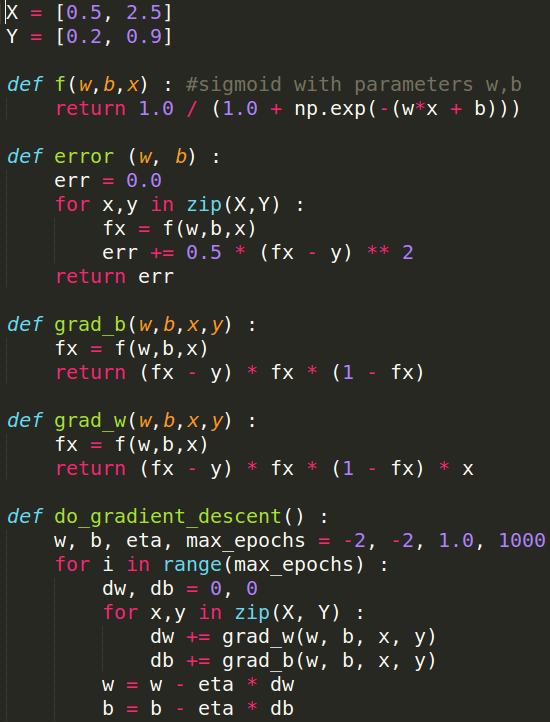
\includegraphics[scale=0.3]{images/module2/pseudo_code_sgd_crop.png}
			\end{figure}
		\end{overlayarea}
		
		\column{0.5\textwidth}
		\begin{overlayarea}{\textwidth}{\textheight}
			\vspace{-0.15in}
			
			%\animategraphics[scale=0.5]{12}{images/module2/sgd0/sgd_error}{0}{99}
			
			\begin{figure}
				\foreach \n in {0,...,99} {%
					\includegraphics<\n>[scale=0.5]{images/module2/sgd0/sgd_error\n.png}
				}
			\end{figure}
		\end{overlayarea}
		
	\end{columns}
\end{frame}

\begin{frame}
	
	\begin{columns}
		
		\column{0.5\textwidth}
		\begin{tikzpicture} 
  \tkzInit[xmin=-1,xmax=4.5,ymax=6]
  \tkzClip[space=1]
    \tkzAxeXY
    \tkzFct[domain=.1:5,samples=200,id=ln,line width=0.5pt,color=red]{x**2 + 1} 
%    \tkzDrawTangentLine[kl=1,kr=5](1)
	\only<2->{\draw[domain=-1:2.2,smooth,variable=\x,red]  plot ({\x}, {\x*\x + 1}); }
    \tkzText[draw=red,fill = red!20](2.75, 6){$f(x)=x^2+1$}
    \only<3->{\derivative{1}{2}{$\Delta x_1$}{$\Delta y_1$}{above}}
    \only<3->{\draw[domain=-1:2.2,smooth,variable=\x,red]  plot ({\x}, {\x*\x + 1}); }
    \only<4->{\derivative{0}{1}{$\Delta x_2$}{$\Delta y_2$}{below}}   
  	
\end{tikzpicture} 

		\column{0.5\textwidth}
		\begin{overlayarea}{\textwidth}{\textheight}
			\begin{itemize}\justifying
				\item<2-> When the curve is steep the gradient ($\frac{\Delta y_1}{\Delta x_1}$) is large
				\item<3-> When the curve is gentle the gradient ($\frac{\Delta y_2}{\Delta x_2}$) is small
				\item<4-> Recall that our weight updates are proportional to the gradient $w = w - \eta \nabla w$
				\item<5-> Hence in the areas where the curve is gentle the updates are small whereas in the areas where the curve is steep the updates are large
			\end{itemize}
			
		\end{overlayarea}
	\end{columns}
	    
\end{frame}

\begin{frame}
	\fontsize{16pt}{7.2}\selectfont
	\begin{itemize}\justifying
		\item \textit{Let's see what happens when we start from a different point}
	\end{itemize}
\end{frame}

\begin{frame}
	
	\begin{columns}
		\column{0.5\textwidth}
		\begin{overlayarea}{\textwidth}{\textheight}
			\begin{itemize}\justifying
				\item<2-> Irrespective of where we start from once we hit a surface which has a gentle slope, the progress slows down
			\end{itemize}
		\end{overlayarea}
		
		\column{0.5\textwidth}
		\begin{overlayarea}{\textwidth}{\textheight}
			\vspace{-0.15in}
			
			%\animategraphics[scale=0.5]{12}{images/module2/sgd0/sgd_error}{0}{99}
			
			\begin{figure}
				\foreach \n in {0,...,129} {%
					\includegraphics<\n>[scale=0.5]{images/module2/sgd0.1/3d_path\n.png}
				}
			\end{figure}
		\end{overlayarea}
		
	\end{columns}
\end{frame}

\begin{frame}
	\myheading{Module 5.3 : Contour Maps}
\end{frame}

\begin{frame}
	\fontsize{16pt}{7.2}\selectfont
	\begin{itemize}\justifying
		\item \textit{Visualizing things in 3d can sometimes become a bit cumbersome}
		      \item<2-> \textit{Can we do a 2d visualization of this traversal along the error surface}
		      \item<3-> \textit{Yes, let's take a look at something known as contours}
	\end{itemize}
	 
\end{frame}

\begin{frame}
	\begin{columns}
		\column{0.5\textwidth}
		\begin{overlayarea}{\textwidth}{\textheight}
			\begin{figure}
				\begin{tikzpicture}
\begin{axis}[axis lines=left, ticks=none,xmax=0.5,ymax=0.5,x label style={at={(axis description cs:0.5,0)},anchor=north},
xlabel={$\theta$}, ylabel={error}]
\addplot[thick,black, no markers, samples=200, domain=-5:0] {-x*exp(x)};
\only<2->{\draw[dashed] (axis cs:-1.88,0.31) -- (axis cs:-0.0,0.31)} ;
\only<2->{\draw[dashed] (axis cs:-2.68,0.21) -- (axis cs:-0.0,0.21)} ;

\end{axis}
\end{tikzpicture}

				\caption{Front view of a 3d error surface}
				
			\end{figure}
		\end{overlayarea}
		
		\column{0.5\textwidth}
		\begin{overlayarea}{\textwidth}{\textheight}
			\only<1-2>{
				\begin{itemize}\justifying
					\item Suppose I take horizontal slices of this error surface at regular intervals along the vertical axis
					\item <2>How would this look from the top-view ?
				\end{itemize}
			}
			
			\only<3->{
				\tikzstyle{neuron}=[circle,draw=blue!50,fill=blue!20,thick,minimum size=10mm]
\tikzstyle{input}=[circle,draw=black!50,fill=black!20,thick,minimum size=6mm]
\begin{tikzpicture}
\node [neuron] (neuron0) at (1,6)  {$\sigma$} ;
\node (input1) at (-1,6)  {$x$};
\node (input0) at (-1,5)  {$1$};
\node (output0) at (3,6)  {$y = f(x)$};
\node (formula) at (0,4) {$f(x)= \frac{1}{1+e^{-(w\cdot x + b)}}$};
\draw [->] (input0) -- (neuron0);
\draw [->] (input1) -- (neuron0);
\draw [->] (neuron0) -- (output0);
\end{tikzpicture}

				\begin{itemize}\justifying
					\item<4-> A small distance between the contours indicates a steep slope along that direction
					\item<5-> A large distance between the contours indicates a gentle slope along that direction
				\end{itemize}
			}
			
		\end{overlayarea}
	\end{columns}
	
\end{frame}

\begin{frame}
	\fontsize{16pt}{7.2}\selectfont
	\begin{itemize}\justifying
		\item \textit{Just to ensure that we understand this properly let us do a few exercises ...}
	\end{itemize}
	 
\end{frame}


\begin{frame}
	\begin{columns}
		\column{0.5\textwidth}
		\begin{overlayarea}{\textwidth}{\textheight}
			\begin{figure}
				\includegraphics<1-2>[scale=0.4]{images/module3/trial/2d_43.png}
				\includegraphics<3-4>[scale=0.4]{images/module3/trial/2d_34.png}
				\includegraphics<5->[scale=0.4]{images/module3/trial/2d_32.png}
			\end{figure}
			\only<1->{Guess the 3d surface}
		\end{overlayarea}
		
		\column{0.5\textwidth}
		\begin{overlayarea}{\textwidth}{\textheight}
			\begin{figure}
				\includegraphics<2>[scale=0.5]{images/module3/trial/3d_43.png}
				\includegraphics<4>[scale=0.5]{images/module3/trial/3d_34.png}
				\includegraphics<6>[scale=0.5]{images/module3/trial/3d_32.png}
			\end{figure}
		\end{overlayarea}
	\end{columns}
	
\end{frame}



\begin{frame}
	\fontsize{16pt}{7.2}\selectfont
	\begin{itemize}\justifying
		\item \textit{Now that we know what are contour maps and how to read them let us go back to our toy example and visualize gradient descent from the point of view of contours...}
	\end{itemize}
	 
\end{frame}


\begin{frame}
	\begin{columns}
		\column{0.5\textwidth}
		\begin{overlayarea}{\textwidth}{\textheight}
			\begin{figure}
				\foreach \n in {0,...,50} {%
					\begin{tikzpicture}
						\sbox0{%
						\includegraphics[scale=0.4]{images/module3/sgd0/sgd_quiver\n.png}
						}%
						\only<\n>{\node[above right,inner sep=0pt] at (0,0)  {\usebox{0}}};%
						\only<\n>{\node[red,font=\small](w) at (0.5\wd0,0.23\ht0) {w}};%
						\only<\n>{\node[red,font=\small](b) at (0,0.67\ht0) {b}};%
						\only<\n>{\draw[->, line width=0.2mm](w)--(0.6\wd0,0.23\ht0)};%
						\only<\n>{\draw[->, line width=0.2mm](b)--(0,0.8\ht0)};%
					\end{tikzpicture}
				}%
			\end{figure}
		\end{overlayarea}
		
		\column{0.5\textwidth}
		\begin{overlayarea}{\textwidth}{\textheight}
			
			\begin{figure}
				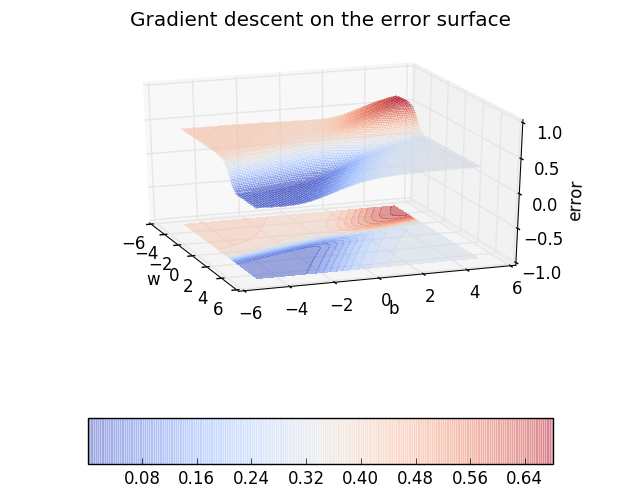
\includegraphics[scale=0.5]{images/module3/sgd0/sgd_error_with_contour.png}
			\end{figure}
			
			
		\end{overlayarea}
	\end{columns}
	
\end{frame}

\begin{frame}
	\begin{columns}
		\column{0.5\textwidth}
		\begin{overlayarea}{\textwidth}{\textheight}
			\begin{figure}
				\foreach \n in {0,...,29} {%
					\pgfmathtruncatemacro\result{int(round(\n+50))}
					\begin{tikzpicture}
						\sbox0{%
						\includegraphics[scale=0.4]{images/module3/sgd0/sgd_quiver\result.png}
						}%
						\only<\n>{\node[above right,inner sep=0pt] at (0,0)  {\usebox{0}}};%
						\only<\n>{\node[red,font=\small](w) at (0.5\wd0,0.23\ht0) {w}};%
						\only<\n>{\node[red,font=\small](b) at (0,0.67\ht0) {b}};%
						\only<\n>{\draw[->, line width=0.2mm](w)--(0.6\wd0,0.23\ht0)};%
						\only<\n>{\draw[->, line width=0.2mm](b)--(0,0.8\ht0)};%
					\end{tikzpicture}
				}%
			\end{figure}
		\end{overlayarea}
		
		\column{0.5\textwidth}
		\begin{overlayarea}{\textwidth}{\textheight}
			
			\begin{figure}
				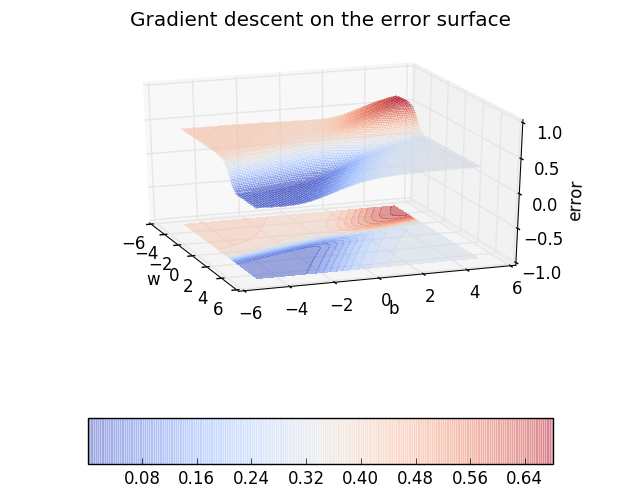
\includegraphics[scale=0.5]{images/module3/sgd0/sgd_error_with_contour.png}
			\end{figure}
			
			
		\end{overlayarea}
	\end{columns}
	
\end{frame}

\begin{frame}
	\myheading{Module 5.4 : Momentum based Gradient Descent}
\end{frame}

\begin{frame}
	\begin{overlayarea}{\textwidth}{\textheight}
		\begin{block}{Some observations about gradient descent}
			\begin{itemize}\justifying
				\item<1-> It takes a lot of time to navigate regions having a gentle slope
				\item<2-> This is because the gradient in these regions is very small
				\item<3-> Can we do something better ?
				\item<4-> Yes, let's take a look at `Momentum based gradient descent'
			\end{itemize}
		\end{block}
	\end{overlayarea}
\end{frame}

%\subsection{Momentum based gradient descent}
\begin{frame}
	\begin{overlayarea}{\textwidth}{\textheight}
		\begin{block}{Intuition}
			\begin{itemize}\justifying
				\item<1-> If I am repeatedly being asked to move in the same direction then I should probably gain some confidence and start taking bigger steps in that direction
				\item<2-> Just as a ball gains momentum while rolling down a slope
			\end{itemize}
		\end{block}
		
		\only<3->{
			\begin{block}{Update rule for momentum based gradient descent}
				\begin{align*}
					update_{t} & = \gamma\cdot update_{t-1} + \eta \nabla w_{t} \\
					w_{t+1}    & = w_{t} - update_{t}                           
				\end{align*}
				
				\begin{itemize}\justifying
					\item<4-> In addition to the current update, also look at the history of updates.
				\end{itemize}
			\end{block}
		}
	\end{overlayarea}
\end{frame}

\begin{frame}
	\begin{overlayarea}{\textwidth}{\textheight}
		\begin{align*}
			update_{t} & = \gamma\cdot update_{t-1} + \eta \nabla w_{t} \\
			w_{t+1}    & = w_{t} - update_{t}                           
		\end{align*}
		
		\vspace{0.1in}
		\begin{align*}
			\onslide<1->{update_{0} & = 0                                                                                                                                                                     \\}
			\onslide<2->{update_{1} & = \gamma\cdot update_{0} + \eta \nabla w_{1} = \eta \nabla w_{1}                                                                                                        \\}
			\onslide<3->{update_{2} & = \gamma\cdot update_{1} + \eta \nabla w_{2} = \gamma\cdot \eta \nabla w_{1} + \eta \nabla w_{2}                                                                        \\}
			\onslide<4->{update_{3} & = \gamma\cdot update_{2} + \eta \nabla w_{3} = \gamma (\gamma \cdot \eta \nabla w_{1} + \eta \nabla w_{2}) + \eta \nabla w_{3}                                          \\}
			\onslide<5->{           & = \gamma\cdot update_{2} + \eta \nabla w_{3} = \gamma^2 \cdot \eta \nabla w_{1} + \gamma \cdot \eta \nabla w_{2} + \eta \nabla w_{3}                                    \\}
			\onslide<6->{update_{4} & = \gamma\cdot update_{3} + \eta \nabla w_{4} = \gamma^3 \cdot \eta \nabla w_{1} + \gamma^2 \cdot \eta \nabla w_{2} + \gamma \cdot \eta \nabla w_{3} + \eta \nabla w_{4} \\}
			\onslide<7->{\vdots\\}
			\onslide<8->{update_{t} & = \gamma\cdot update_{t-1} + \eta \nabla w_{t} = \gamma^{t-1} \cdot \eta \nabla w_{1} + \gamma^{t-2} \cdot \eta \nabla w_{1} +  ... + \eta \nabla w_{t}                 \\}
		\end{align*}
		
		
	\end{overlayarea}
	
\end{frame}

\begin{frame}
	\begin{columns}
		\column{0.5\textwidth}
		\begin{overlayarea}{\textwidth}{\textheight}
			\vspace{-0.15in}
			\begin{figure}
				\includegraphics[scale=0.3]{images/module4/pseudo_code_mom_crop.png}
			\end{figure}
		\end{overlayarea}
		
		\column{0.5\textwidth}
		\begin{overlayarea}{\textwidth}{\textheight}
			\vspace{-0.15in}
			\foreach \n in {0,...,20} {%
				\begin{tikzpicture}
					\sbox0{\includegraphics[scale=0.4]{images/module4/mom1/2d_path\n.png}}% get width and height
					\only<\n>{\node[above right,inner sep=0pt] at (0,0)  {\usebox{0}}};
					\only<\n>{\node[red](w) at (0.5\wd0,0) {w}};
					\only<\n>{\node[red](b) at (0,0.67\ht0) {b}};
					\only<\n>{\draw[->, line width=0.2mm](w)--(0.6\wd0,0)};
					\only<\n>{\draw[->, line width=0.2mm](b)--(0,0.8\ht0)};
				\end{tikzpicture}
			}
			% \sbox0{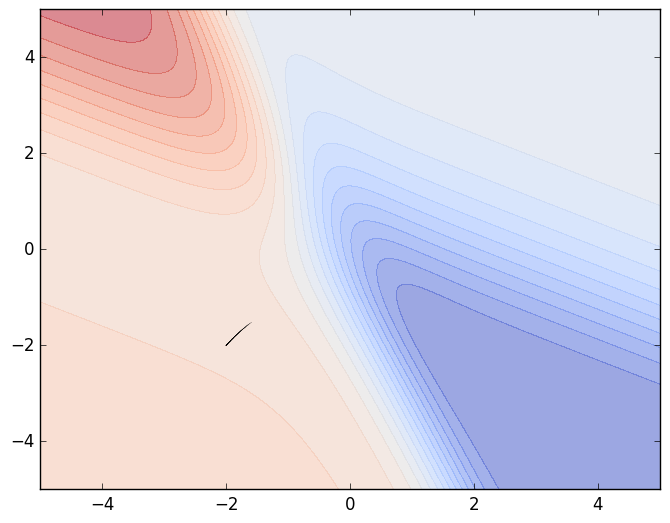
\includegraphics[scale=0.4]{images/module4/mom1/2d_path0.png}}% get width and height
		\end{overlayarea}
		
	\end{columns}
\end{frame}

\begin{frame}
	\begin{overlayarea}{\textwidth}{\textheight}
		\begin{block}{Some observations and questions}
			\begin{itemize}\justifying
				\item Even in the regions having gentle slopes, momentum based gradient descent is able to take large steps because the momentum carries it along
				      \item<2-> Is moving fast always good? Would there be a situation where momentum would cause us to run pass our goal?
				      \item<3-> Let us change our input data so that we end up with a different error surface and then see what happens ... 
			\end{itemize}
		\end{block}
	\end{overlayarea}
\end{frame}


\begin{frame}
	\begin{columns}
		\column{0.5\textwidth}
		\begin{overlayarea}{\textwidth}{\textheight}
			\begin{itemize}\justifying
				\item<2-> In this case, the error is high on either side of the minima valley
				\item<3-> Could momentum be detrimental in such cases... let's see....
			\end{itemize}
		\end{overlayarea}
		
		\column{0.5\textwidth}
		\begin{overlayarea}{\textwidth}{\textheight}
			\begin{figure}
				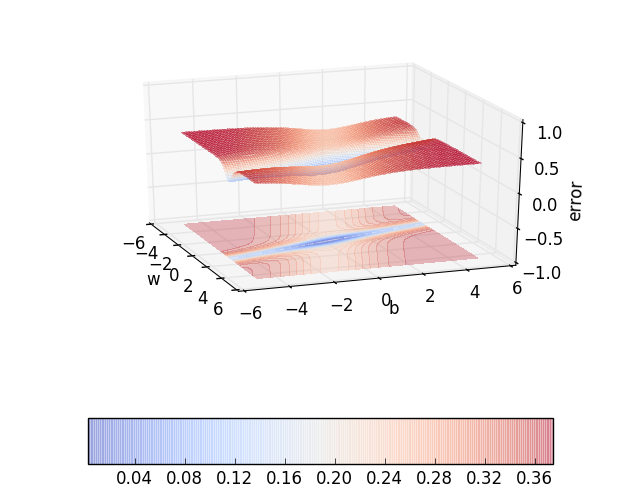
\includegraphics[scale=0.5]{images/module4/error_surface2.png}
			\end{figure}
		\end{overlayarea}
	\end{columns}
	
\end{frame}

\begin{frame}
	\begin{columns}
		\column{0.5\textwidth}
		\begin{overlayarea}{\textwidth}{\textheight}
			\begin{itemize}\justifying
				\item<37-> Momentum based gradient descent oscillates in and out of the minima valley as the momentum carries it out of the valley
				\item<38-> Takes a lot of \textit{u}-turns before finally converging 
				\item<39-> Despite these \textit{u}-turns it still converges faster than vanilla gradient descent
				\item<40-> After $100$ iterations momentum based method has reached an error of $0.00001$ whereas vanilla gradient descent is still stuck at an error of $0.36$ 
			\end{itemize}
		\end{overlayarea}
		
		\column{0.5\textwidth}
		\begin{overlayarea}{\textwidth}{\textheight}
			\begin{figure}
				\foreach \n in {0,...,40} {%
					\begin{tikzpicture}
						\sbox0{\includegraphics[scale=0.4]{images/module4/mom2/2d_path\n.png}}% get width and height
						\only<\n>{\node[above right,inner sep=0pt] at (0,0)  {\usebox{0}}};
						\only<\n>{\node[red](w) at (0.5\wd0,0.23\ht0) {w}};
						\only<\n>{\node[red](b) at (0,0.67\ht0) {b}};
						\only<\n>{\draw[->, line width=0.2mm](w)--(0.6\wd0,0.23\ht0)};
						\only<\n>{\draw[->, line width=0.2mm](b)--(0,0.8\ht0)};
					\end{tikzpicture}
				}
			\end{figure}
		\end{overlayarea}
	\end{columns}
	
\end{frame}

\begin{frame}
	\fontsize{16pt}{7.2}\selectfont
	\textit{Let's look at a 3d visualization and a different geometric perspective of the same thing...}
\end{frame}

\begin{frame}
	\begin{columns}
		\column{0.52\textwidth}
		\begin{overlayarea}{\textwidth}{\textheight}
			\begin{figure}
				\centering
				\foreach \n in {0,...,40} {%
					\includegraphics<\n>[scale=0.7]{images/module4/mom2/3d_path\n.png}
				}
			\end{figure}
		\end{overlayarea}
		
		\column{0.48\textwidth}
		\begin{overlayarea}{\textwidth}{\textheight}
			\begin{figure}
				\foreach \n in {0,...,40} {%
					\includegraphics<\n>[scale=0.4]{images/module4/mom2/sigmoid\n.png}
				}
			\end{figure}
		\end{overlayarea}
	\end{columns}
	
\end{frame}


\begin{frame}
	\myheading{Module 5.5 : Nesterov Accelerated Gradient Descent}
\end{frame}

\begin{frame}
	\begin{overlayarea}{\textwidth}{\textheight}
		\begin{block}{Question}
			\begin{itemize}\justifying
				\item Can we do something  to reduce these oscillations ?
				      \item<2-> Yes, let's look at Nesterov accelerated gradient
			\end{itemize}
		\end{block}
	\end{overlayarea}
\end{frame}

%\subsection{Nesterov accelerated gradient descent}
\begin{frame}
	
	\begin{overlayarea}{\textwidth}{\textheight}
		\vspace{-0.2in}
		\begin{block}{Intuition}
			\begin{itemize}\justifying
				\item<1-> Look before you leap
				\item<2-> Recall that $update_{t} = \gamma\cdot update_{t-1} + \eta \nabla w_{t}$
				\item<3-> So we know that we are going to move by at least by $\gamma\cdot update_{t-1}$ and then a bit more by $\eta \nabla w_{t}$
				\item<4-> Why not calculate the gradient ($\nabla w_{look\_ahead}$) at this partially updated value of $w$ ($w_{look\_ahead} = w_{t} - \gamma\cdot update_{t-1}$)  instead of calculating it using the current value $w_{t}$
			\end{itemize}
		\end{block}
		
		\only<5->{
			\vspace{-0.1in}
			\begin{block}{Update rule for NAG}
				\begin{align*}
					w_{_{look\_ahead}} & = w_{t} - \gamma\cdot update_{t-1}                          \\
					update_t           & = \gamma\cdot update_{t-1} + \eta \nabla w_{_{look\_ahead}} \\
					w_{t+1}            & = w_{t} - update_{t}                                        
				\end{align*}
				We will have similar update rule for $b_t$
			\end{block}
		}
	\end{overlayarea}
\end{frame}

\begin{frame}
	%Mitesh: replace pseudo_code_sgd_crop by code for momentum based sgd
	% replace sgd_error\n.png by mom_error\n.png
	\begin{columns}
		\column{0.5\textwidth}
		\begin{overlayarea}{\textwidth}{\textheight}
			\vspace{-0.15in}
			\begin{figure}
				\includegraphics[scale=0.3]{images/module5/pseudo_code_nag_crop.png}
			\end{figure}
		\end{overlayarea}
		
		\column{0.5\textwidth}
		\begin{overlayarea}{\textwidth}{\textheight}
			\vspace{-0.15in}
			\begin{figure}
				\foreach \n in {0,...,40} {%
					\begin{tikzpicture}
						\sbox0{\includegraphics[scale=0.4]{images/module5/nag2/2d_path\n.png}}% get width and height
						\only<\n>{\node[above right,inner sep=0pt] at (0,0)  {\usebox{0}}};
						\only<\n>{\node[red](w) at (0.5\wd0,0.23\ht0) {w}};
						\only<\n>{\node[red](b) at (0,0.67\ht0) {b}};
						\only<\n>{\draw[->, line width=0.2mm](w)--(0.6\wd0,0.23\ht0)};
						\only<\n>{\draw[->, line width=0.2mm](b)--(0,0.8\ht0)};
					\end{tikzpicture}
				}
			\end{figure}
		\end{overlayarea}
	\end{columns}
\end{frame}

\begin{frame}
\end{frame}

\begin{frame}
	\begin{overlayarea}{\textwidth}{\textheight}
		\begin{block}{Observations about NAG}
			\begin{itemize}\justifying
				\item<1-> Looking ahead helps NAG in correcting its course quicker than momentum based gradient descent
				\item<2-> Hence the oscillations are smaller and the chances of escaping the minima valley also smaller
			\end{itemize}
		\end{block}
	\end{overlayarea}
\end{frame}

\begin{frame}
	\myheading{Module 5.6 : Stochastic And Mini-Batch Gradient Descent}
\end{frame}

\begin{frame}
	\fontsize{16pt}{7.2}\selectfont
	\textit{Let's digress a bit and talk about the stochastic version of these algorithms...}
\end{frame}

\begin{frame}
	\begin{columns}
		\column{0.4\textwidth}
		\begin{overlayarea}{\textwidth}{\textheight}
			\vspace{-0.15in}
			\begin{figure}
				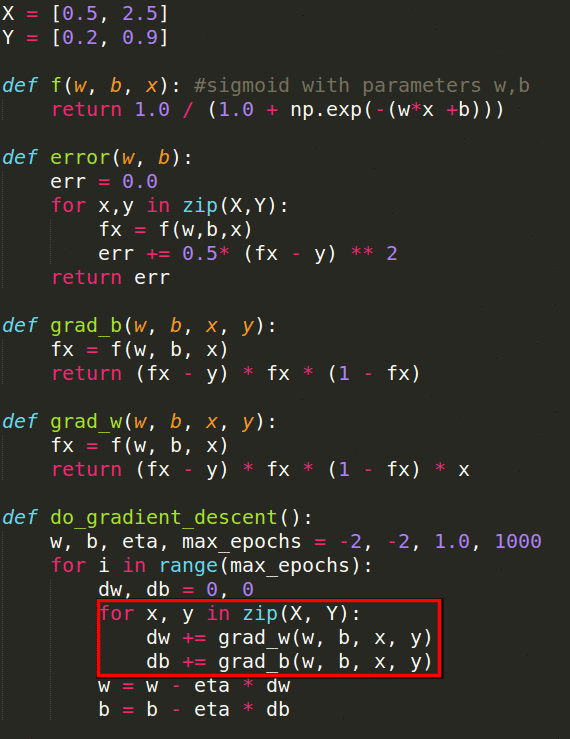
\includegraphics[scale=0.3]{images/module6/pseudo_code_sgd_crop_highlight.png}
			\end{figure}
		\end{overlayarea}
		
		\column{0.6\textwidth}
		\begin{overlayarea}{\textwidth}{\textheight}
			
			\begin{itemize}\justifying
				\item<2-> Notice that the algorithm goes over the entire data once before updating the parameters
				\item<3-> \only<3->{Why?} \onslide<4->{Because this is the true gradient of the loss as derived earlier (sum of the gradients of the losses corresponding to each data point)}
				
				\item<5-> \onslide<5->{No approximation.} \onslide<6->{Hence, theoretical guarantees hold (in other words each step guarantees that the loss will decrease)}
				\item<7-> What's the flipside? \onslide<8->{Imagine we have a million points in the training data.} \onslide<9->{To make 1 update to $w, b$ the algorithm makes a million calculations.} \onslide<10->{Obviously very slow!!}
				\item<11-> \only<11->{Can we do something better ?} \onslide<12->{Yes, let's look at stochastic gradient descent}
			\end{itemize}
			
			
		\end{overlayarea}
		
	\end{columns}
\end{frame}

\begin{frame}
	\begin{columns}
		\column{0.4\textwidth}
		\begin{overlayarea}{\textwidth}{\textheight}
			\vspace{-0.15in}
			\begin{figure}
				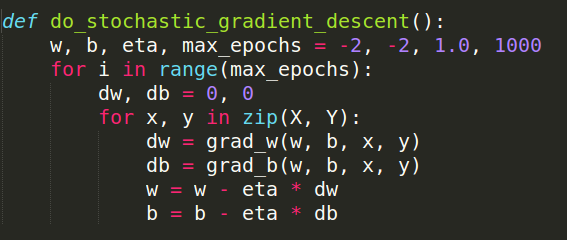
\includegraphics[scale=0.3]{images/module6/pseudo_code_stoch_gd_crop.png}
			\end{figure}
			
			\only<1-3>{
				\begin{figure}
					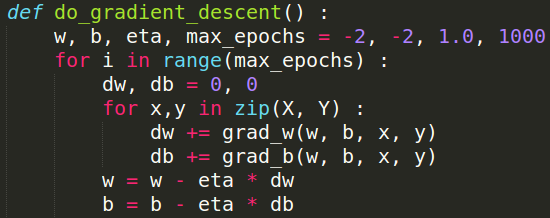
\includegraphics[scale=0.3]{images/module6/pseudo_code_sgd_crop_small.png}
				\end{figure}
			}
			
			\begin{itemize}\justifying 
				\item<6-> Stochastic because we are estimating the total gradient based on a single data point. \onslide<7->{Almost like tossing a coin only once and estimating P(heads).}
			\end{itemize} 
		\end{overlayarea}
		
		
		\column{0.6\textwidth}
		\begin{overlayarea}{\textwidth}{\textheight}
			
			\begin{itemize}\justifying
				\item<2-> Notice that the algorithm updates the parameters for every single data point
				\item<3-> Now if we have a million data points we will make a million updates in each epoch (1 epoch = 1 pass over the data; 1 step = 1 update)
				\item<4-> What is the flipside ? \onslide<5->{It is an approximate (rather stochastic) gradient}
				\item<8-> No guarantee that each step will decrease the loss
				\item<9-> Let's see this algorithm in action when we have a few data points
			\end{itemize}
			
		\end{overlayarea}
		
	\end{columns}
\end{frame}

\begin{frame}
	\begin{columns}
		\column{0.53\textwidth}
		\begin{overlayarea}{\textwidth}{\textheight}
			% \begin{itemize}\justifying
			% 	\item<37-> We see many oscillations. Why ? \onslide<38->{ Because we are making greedy decisions.}
			% 	\item<39-> Each point is trying to push the parameters in a direction most favorable to it \onslide<40->{(without being aware of how this affects other points)}
			% 	\item<41-> A parameter update which is locally favorable to one point may harm other points \onslide<42->{(its almost as if the data points are competing with each other)}
			% 	%\item<7-> Indeed we see that there is no guarantee that each local greedy move reduces the global error
			% 	\item<43-> Can we reduce the oscillations by improving our stochastic estimates of the gradient \onslide<44->{(currently estimated from just 1 data point at a time)}
			% 	\item<45-> Yes, let's look at mini-batch gradient descent
			% \end{itemize}
		\end{overlayarea}
		
		\column{0.47\textwidth}
		\begin{overlayarea}{\textwidth}{\textheight}
			
			\begin{figure}[ht]
				%\foreach[count=\i, evaluate=\i as \x using int(\i+5)] \n in {1,...,45}
				%{
				\foreach \n in {0,...,30} {%
					\pgfmathtruncatemacro\result{int(round(\n * 5))}
					\begin{tikzpicture}
						\sbox0{%
						\includegraphics[scale=0.414]{images/module6/stoch_gd3/2d_path\result.png}%
						}%
						\only<\n>{\node[above right,inner sep=0pt] at (0,0)  {\usebox{0}}};%
						\only<\n>{\node[red,font=\small](w) at (0.5\wd0,0.23\ht0) {w}};%
						\only<\n>{\node[red,font=\small](b) at (0,0.67\ht0) {b}};%
						\only<\n>{\draw[->, line width=0.2mm](w)--(0.6\wd0,0.23\ht0)};%
						\only<\n>{\draw[->, line width=0.2mm](b)--(0,0.8\ht0)};%
					\end{tikzpicture}
				}%
				
			\end{figure}
		\end{overlayarea}
	\end{columns}
\end{frame}

\begin{frame}
	\begin{columns}
		\column{0.53\textwidth}
		\begin{overlayarea}{\textwidth}{\textheight}
			\begin{itemize}\justifying
				\item<7-> We see many oscillations. Why ? \onslide<8->{ Because we are making greedy decisions.}
				\item<9-> Each point is trying to push the parameters in a direction most favorable to it \onslide<10->{(without being aware of how this affects other points)}
				\item<11-> A parameter update which is locally favorable to one point may harm other points \onslide<12->{(its almost as if the data points are competing with each other)}
				%\item<7-> Indeed we see that there is no guarantee that each local greedy move reduces the global error
				\item<13-> Can we reduce the oscillations by improving our stochastic estimates of the gradient \onslide<14->{(currently estimated from just 1 data point at a time)}
				\item<15-> Yes, let's look at mini-batch gradient descent
			\end{itemize}
		\end{overlayarea}
		
		\column{0.47\textwidth}
		\begin{overlayarea}{\textwidth}{\textheight}
			
			\begin{figure}[ht]
				%\foreach[count=\i, evaluate=\i as \x using int(\i+5)] \n in {1,...,45}
				%{
				\foreach \n in {0,...,15} {%
					\pgfmathtruncatemacro\result{int(round((\n+30) * 5))}
					\begin{tikzpicture}
						\sbox0{%
						\includegraphics[scale=0.414]{images/module6/stoch_gd3/2d_path\result.png}%
						}%
						\only<\n>{\node[above right,inner sep=0pt] at (0,0)  {\usebox{0}}};%
						\only<\n>{\node[red,font=\small](w) at (0.5\wd0,0.23\ht0) {w}};%
						\only<\n>{\node[red,font=\small](b) at (0,0.67\ht0) {b}};%
						\only<\n>{\draw[->, line width=0.2mm](w)--(0.6\wd0,0.23\ht0)};%
						\only<\n>{\draw[->, line width=0.2mm](b)--(0,0.8\ht0)};%
					\end{tikzpicture}
				}%
				
			\end{figure}
		\end{overlayarea}
	\end{columns}
\end{frame}


\begin{frame}
	\begin{columns}
		\column{0.5\textwidth}
		\begin{overlayarea}{\textwidth}{\textheight}
			\vspace{-0.15in}
			\begin{figure}
				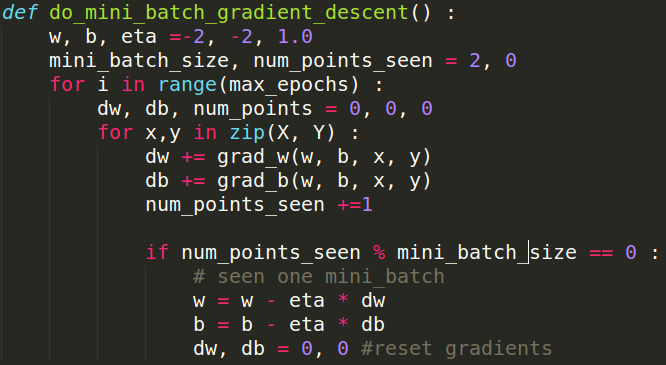
\includegraphics[scale=0.3]{images/module6/pseudo_code_mini_batch_gd_crop.png}
			\end{figure}
			
			\only<1-3>{
				\begin{figure}
					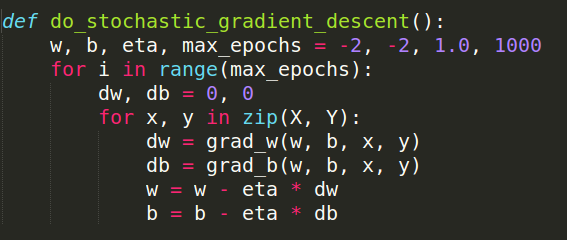
\includegraphics[scale=0.3]{images/module6/pseudo_code_stoch_gd_crop.png}
				\end{figure}
			}
		\end{overlayarea}
		
		
		\column{0.5\textwidth}
		\begin{overlayarea}{\textwidth}{\textheight}
			
			\begin{itemize}\justifying
				\item<1-> Notice that the algorithm updates the parameters after it sees $mini\_batch\_size$ number of data points
				\item<2-> The stochastic estimates are now slightly better
				\item<3-> Let's see this algorithm in action when we have k = 2
			\end{itemize}
			
		\end{overlayarea}
		
	\end{columns}
\end{frame}


\begin{frame}
	\begin{columns}
		\column{0.57\textwidth}
		\begin{overlayarea}{\textwidth}{\textheight}
			% \begin{itemize}\justifying
			% 	\item<39-> Even with a batch size of k=2 the oscillations have reduced slightly. \onslide<40->{Why ?} 
			% 	\item<41-> Because we now have slightly better estimates of the gradient \onslide<42->{[analogy: we are now tossing the coin k=2 times to estimate P(heads)]}
			% 	\item<43-> The higher the value of k the more accurate are the estimates 
			% 	\item<44-> In practice, typical values of k are 16, 32, 64
			% 	\item<45-> Of course, there are still oscillations and they will always be there as long as we are using an approximate gradient as opposed to the true gradient
			% \end{itemize}
		\end{overlayarea}
		
		\column{0.43\textwidth}
		\begin{overlayarea}{\textwidth}{\textheight}
			\begin{figure}
				\foreach \n in {0,...,25} {%
					\pgfmathtruncatemacro\result{int(round(\n * 2))}
					\begin{tikzpicture}
						\sbox0{\includegraphics[scale=0.38]{images/module6/mini_batch_gd5/2d_path\result.png}}% get width and height
						\only<\n>{\node[above right,inner sep=0pt] at (0,0)  {\usebox{0}}};
						\only<\n>{\node[red,font=\small](w) at (0.5\wd0,0.23\ht0) {w}};
						\only<\n>{\node[red,font=\small](b) at (0,0.67\ht0) {b}};
						\only<\n>{\draw[->, line width=0.2mm](w)--(0.6\wd0,0.23\ht0)};
						\only<\n>{\draw[->, line width=0.2mm](b)--(0,0.8\ht0)};
					\end{tikzpicture}
				}
			\end{figure}
		\end{overlayarea}
	\end{columns}
\end{frame}


\begin{frame}
	\begin{columns}
		\column{0.57\textwidth}
		\begin{overlayarea}{\textwidth}{\textheight}
			\begin{itemize}\justifying
				\item<20-> Even with a batch size of k=2 the oscillations have reduced slightly. \onslide<21->{Why ?} 
				\item<22-> Because we now have slightly better estimates of the gradient \onslide<23->{[analogy: we are now tossing the coin k=2 times to estimate P(heads)]}
				\item<24-> The higher the value of k the more accurate are the estimates 
				\item<25-> In practice, typical values of k are 16, 32, 64
				\item<26-> Of course, there are still oscillations and they will always be there as long as we are using an approximate gradient as opposed to the true gradient
			\end{itemize}
		\end{overlayarea}
		
		\column{0.43\textwidth}
		\begin{overlayarea}{\textwidth}{\textheight}
			\begin{figure}
				\foreach \n in {0,...,20} {%
					\pgfmathtruncatemacro\result{int(round((\n+25) * 2))}
					\begin{tikzpicture}
						\sbox0{\includegraphics[scale=0.38]{images/module6/mini_batch_gd5/2d_path\result.png}}% get width and height
						\only<\n>{\node[above right,inner sep=0pt] at (0,0)  {\usebox{0}}};
						\only<\n>{\node[red,font=\small](w) at (0.5\wd0,0.23\ht0) {w}};
						\only<\n>{\node[red,font=\small](b) at (0,0.67\ht0) {b}};
						\only<\n>{\draw[->, line width=0.2mm](w)--(0.6\wd0,0.23\ht0)};
						\only<\n>{\draw[->, line width=0.2mm](b)--(0,0.8\ht0)};
					\end{tikzpicture}
				}
				\begin{tikzpicture}
						\sbox0{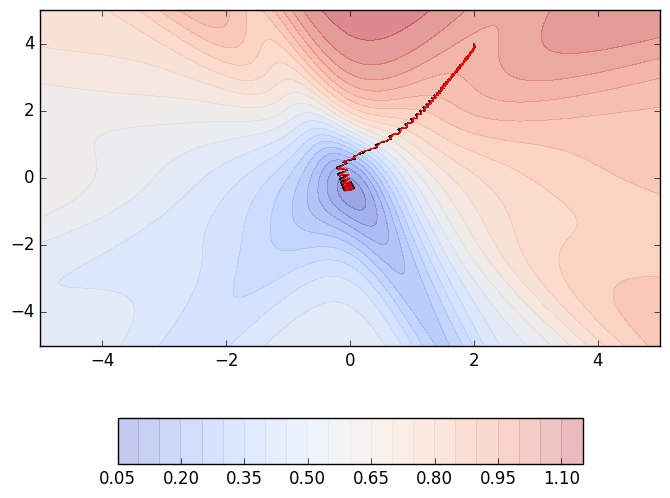
\includegraphics[scale=0.38]{images/module6/mini_batch_gd5/2d_path90.png}}% get width and height
						\only<21->{\node[above right,inner sep=0pt] at (0,0)  {\usebox{0}}};
						\only<21->{\node[red,font=\small](w) at (0.5\wd0,0.23\ht0) {w}};
						\only<21->{\node[red,font=\small](b) at (0,0.67\ht0) {b}};
						\only<21->{\draw[->, line width=0.2mm](w)--(0.6\wd0,0.23\ht0)};
						\only<21->{\draw[->, line width=0.2mm](b)--(0,0.8\ht0)};
					\end{tikzpicture}
			\end{figure}
		\end{overlayarea}
	\end{columns}
\end{frame}


\begin{frame}
	\begin{overlayarea}{\textwidth}{\textheight}
		\begin{block}{Some things to remember ....}
			\begin{itemize}\justifying
				\item 1 epoch = one pass over the entire data
				\item 1 step = one update of the parameters
				\item N = number of data points
				\item B = Mini batch size
				      
				      \begin{table}
				      	\begin{tabular}{cc}
				      		\hline\hline
				      		Algorithm                        & \# of steps in 1 epoch   \\
				      		\hline
				      		Vanilla (Batch) Gradient Descent & \only<2->{1}             \\
				      		Stochastic Gradient Descent      & \only<3->{N}             \\
				      		Mini-Batch Gradient Descent      & \only<4->{$\frac{N}{B}$} \\
				      		\hline\hline
				      	\end{tabular}
				      \end{table}
				      
			\end{itemize}
		\end{block}
	\end{overlayarea}
\end{frame}

\begin{frame}
	\fontsize{16pt}{7.2}\selectfont
	\textit{Similarly, we can have stochastic versions of Momentum based gradient descent and Nesterov accelerated based gradient descent}
\end{frame}


\begin{frame}
	\begin{columns}
		\column{0.5\textwidth}
		\begin{overlayarea}{\textwidth}{\textheight}
			\begin{figure}
				\includegraphics[scale=0.3]{images/module6/pseudo_code_mom_crop.png}
			\end{figure}
		\end{overlayarea}
		
		\column{0.5\textwidth}
		\begin{overlayarea}{\textwidth}{\textheight}
			\begin{figure}
				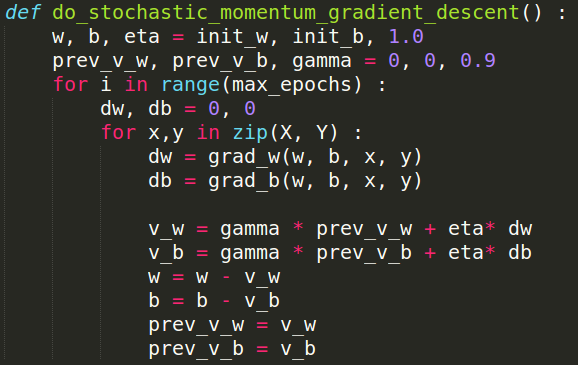
\includegraphics[scale=0.3]{images/module6/pseudo_code_stoch_mom_crop.png}
			\end{figure}
		\end{overlayarea}
	\end{columns}
\end{frame}

\begin{frame}
	\begin{columns}
		\column{0.5\textwidth}
		\begin{overlayarea}{\textwidth}{\textheight}
			\begin{figure}
				\includegraphics[scale=0.3]{images/module6/pseudo_code_nag_crop.png}
			\end{figure}
		\end{overlayarea}
		
		\column{0.5\textwidth}
		\begin{overlayarea}{\textwidth}{\textheight}
			\begin{figure}
				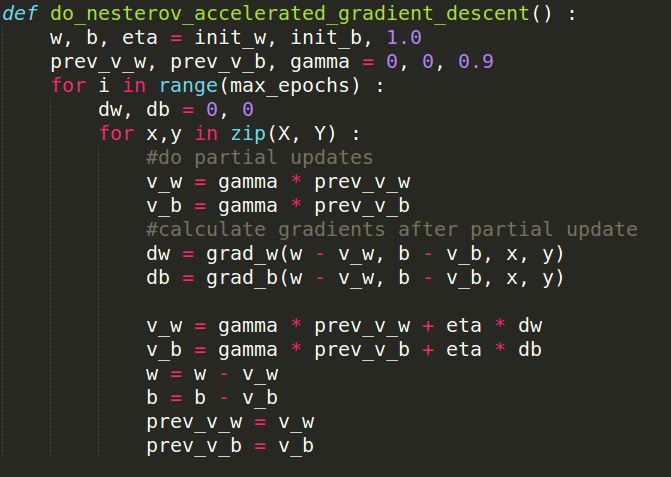
\includegraphics[scale=0.3]{images/module6/pseudo_code_stoch_nag_crop.png}
			\end{figure}
		\end{overlayarea}
	\end{columns}
\end{frame}



\begin{frame}
	\begin{columns}
		
		\column{0.6\textwidth}
		\begin{overlayarea}{\textwidth}{\textheight}
			
			\begin{itemize}\justifying 
				\item<2-> While the stochastic versions of both Momentum [red] and NAG [blue] exhibit oscillations the relative advantage of NAG over Momentum still holds \onslide<3->{(i.e., NAG takes relatively shorter u-turns)}
				\item<4-> Further both of them are faster than stochastic gradient descent \onslide<5->{(after 60 steps, stochastic gradient descent [black - top figure] still exhibits a very high error whereas NAG and Momentum are close to convergence)}
			\end{itemize} 
		\end{overlayarea}
		
		\column{0.4\textwidth}
		\begin{overlayarea}{\textwidth}{\textheight}
			\vspace{-0.1in}
			\begin{tikzpicture}
				\sbox0{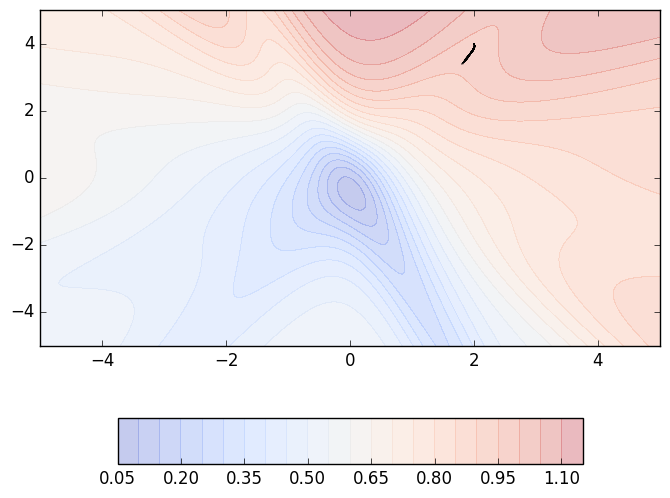
\includegraphics[scale=0.3]{images/module6/stoch_gd6/2d_path60.png}}% get width and height
				\node[above right,inner sep=0pt] at (0,0)  {\usebox{0}};
				\node[red](w) at (0.5\wd0,0.23\ht0) {w};
				\node[red](b) at (0,0.67\ht0) {b};
				\draw[->, line width=0.2mm](w)--(0.6\wd0,0.23\ht0);
				\draw[->, line width=0.2mm](b)--(0,0.8\ht0);
			\end{tikzpicture}
			
			\vspace{-0.05in}
			\begin{tikzpicture}
				\sbox0{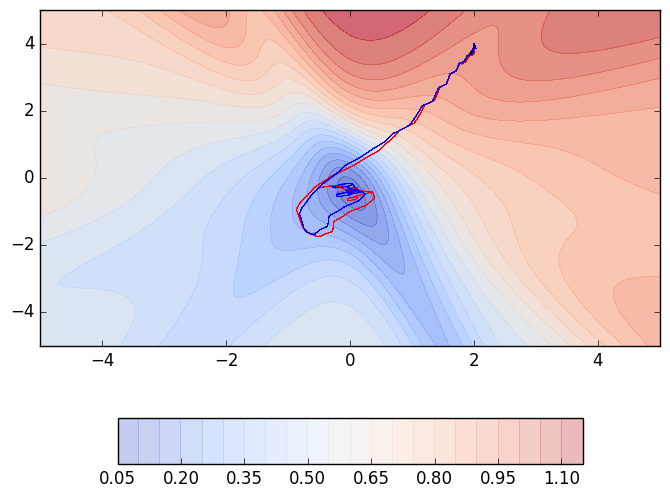
\includegraphics[scale=0.3]{images/module6/stoch_nag6/2d_path60.png}}% get width and height
				\node[above right,inner sep=0pt] at (0,0)  {\usebox{0}};
				\node[red](w) at (0.5\wd0,0.23\ht0) {w};
				\node[red](b) at (0,0.67\ht0) {b};
				\draw[->, line width=0.2mm](w)--(0.6\wd0,0.23\ht0);
				\draw[->, line width=0.2mm](b)--(0,0.8\ht0);
			\end{tikzpicture}
		\end{overlayarea}
		
	\end{columns}
\end{frame}

\begin{frame}
	\fontsize{16pt}{7.2}\selectfont
	\textit{And, of course, you can also have the mini batch version of Momentum and NAG...\onslide<2->{I leave that as an exercise :-)}}
\end{frame}

\begin{frame}
	\myheading{Module 5.7 : Tips for Adjusting learning Rate and Momentum}
\end{frame}

\begin{frame}
	\fontsize{16pt}{7.2}\selectfont
	\textit{Before moving on to advanced optimization algorithms let us revisit the problem of learning rate in gradient descent}
\end{frame}

\begin{frame}
	\begin{columns}
		\column{0.57\textwidth}
		\begin{overlayarea}{\textwidth}{\textheight}
			\begin{itemize}\justifying
				\item One could argue that we could have solved the problem of navigating gentle slopes by setting the learning rate high (i.e., blow up the small gradient by multiplying it with a large $\eta$) 
				      \item<2-> Let us see what happens if we set the learning rate to 10
				      \item<18-> On the regions which have a steep slope, the already large gradient blows up further
				      \item<19-> It would be good to have a learning rate which could adjust to the gradient ... \onslide<20->{we will see a few such algorithms soon}
			\end{itemize}
		\end{overlayarea}
		
		\column{0.43\textwidth}
		\begin{overlayarea}{\textwidth}{\textheight}
			\begin{figure}
				\foreach \n in {0,...,20} {%
					\pgfmathtruncatemacro\result{int(round(\n + 2))}
					\begin{tikzpicture}
						\sbox0{\includegraphics[scale=0.38]{images/module7/sgd0.3/2d_path\result.png}}% get width and height
						\only<\n>{\node[above right,inner sep=0pt] at (0,0)  {\usebox{0}}};
						\only<\n>{\node[red,font=\small](w) at (0.5\wd0,0.23\ht0) {w}};
						\only<\n>{\node[red,font=\small](b) at (0,0.67\ht0) {b}};
						\only<\n>{\draw[->, line width=0.2mm](w)--(0.6\wd0,0.23\ht0)};
						\only<\n>{\draw[->, line width=0.2mm](b)--(0,0.8\ht0)};
					\end{tikzpicture}
				}
			\end{figure}
		\end{overlayarea}
	\end{columns}
\end{frame}

\begin{frame}
	\begin{overlayarea}{\textwidth}{\textheight}
		\onslide<1->{
			\begin{block}{Tips for initial learning rate ?}
				\onslide<2->{
					\begin{itemize}\justifying
						\item<2-> Tune learning rate \onslide<2->{[Try different values on a log scale: 0.0001, 0.001, 0.01, 0.1. 1.0]}
						\item<3-> Run a few epochs with each of these and figure out a learning rate which works best
						\item<4-> Now do a finer search around this value  [for example, if the best learning rate was 0.1 then now try some values around it: 0.05, 0.2, 0.3]
						\item<5-> Disclaimer: these are just heuristics ... no clear winner strategy
					\end{itemize}
				}
			\end{block}
		}
	\end{overlayarea}
\end{frame}

\begin{frame}
	\begin{overlayarea}{\textwidth}{\textheight}
		\only<1->{
			\begin{block}{Tips for annealing learning rate}
				\onslide<2->{
					\begin{itemize}\justifying
						\item<2-> \textbf{Step Decay:}
						\begin{itemize}\justifying
							\item<3-> Halve the learning rate after every 5 epochs or
							\item<4-> Halve the learning rate after an epoch if the validation error is more than what it was at the end of the previous epoch 
						\end{itemize}
						\item<5-> \textbf{Exponential Decay:} $\eta = \eta_{0}^{-kt}$ where $\eta_{0}$ and $k$ are hyperparameters and $t$ is the step number
						\item<6-> \textbf{1/t Decay:} $\eta = \frac{\eta_{0}}{1 + kt}$ where $\eta_{0}$ and $k$ are hyperparameters and $t$ is the step number
					\end{itemize}
				}
			\end{block}
		}
	\end{overlayarea}
\end{frame}


\begin{frame}
	\begin{overlayarea}{\textwidth}{\textheight}
		\begin{block}{Tips for momentum}
			\begin{itemize}\justifying
				\item The following schedule was suggested by Sutskever \textit{et. al.}, 2013
				      \begin{align*}
				      	\gamma_t = min (1 - 2^{-1 - log_2(\lfloor {t/250} \rfloor + 1)}, \gamma_{max})      \\
				      	\intertext{where, $\gamma_{max}$ was chosen from \{0.999, 0.995, 0.99, 0.9, 0\}} 
				      \end{align*}
			\end{itemize}
		\end{block}
	\end{overlayarea}
\end{frame}

\begin{frame}
	\myheading{Module 5.8 : Line Search}
\end{frame}

\begin{frame}
	\fontsize{16pt}{7.2}\selectfont
	\textit{Just one last thing before we move on to some other algorithms ...}
\end{frame}


\begin{frame}
	\begin{columns}
		\column{0.5\textwidth}
		\begin{overlayarea}{\textwidth}{\textheight}
			\begin{itemize}\justifying
				\item<1-> In practice, often a line search is done to find a relatively better value of $\eta$
				\item<3-> Update $w$ using different values of $\eta$
				\item<4-> Now retain that updated value of $w$ which gives the lowest loss
				\item<5-> Esentially at each step we are trying to use the best $\eta$ value from the available choices
				\item<6-> What's the flipside? \onslide<7->{We are doing many more computations in each step}
				\item<8-> We will come back to this when we talk about second order optimization methods
			\end{itemize}
		\end{overlayarea}
		
		\column{0.5\textwidth}
		\begin{overlayarea}{\textwidth}{\textheight}
			\begin{figure}
				\includegraphics<2->[scale=0.3]{images/module8/pseudo_code_line_search_sgd_crop.png}
			\end{figure}
		\end{overlayarea}
	\end{columns}
\end{frame}

\begin{frame}
	\begin{columns}
		\column{0.57\textwidth}
		\begin{overlayarea}{\textwidth}{\textheight}
			\begin{itemize}\justifying
				\item<1-> Let us see line search in action
				\item<17-> Convergence is faster than vanilla gradient descent 
				\item<18-> We see some oscillations, \onslide<19->{but note that these oscillations are different from what we see in momentum and NAG} 
			\end{itemize}
		\end{overlayarea}
		
		\column{0.43\textwidth}
		\begin{overlayarea}{\textwidth}{\textheight}
			\begin{figure}
				\foreach \n in {0,...,20} {%
					\begin{tikzpicture}
						\sbox0{\includegraphics[scale=0.38]{images/module8/line_search_gd0/2d_path\n.png}}% get width and height
						\only<\n>{\node[above right,inner sep=0pt] at (0,0)  {\usebox{0}}};
						\only<\n>{\node[red,font=\small](w) at (0.5\wd0,0.23\ht0) {w}};
						\only<\n>{\node[red,font=\small](b) at (0,0.67\ht0) {b}};
						\only<\n>{\draw[->, line width=0.2mm](w)--(0.6\wd0,0.23\ht0)};
						\only<\n>{\draw[->, line width=0.2mm](b)--(0,0.8\ht0)};
					\end{tikzpicture}
				}
			\end{figure}
		\end{overlayarea}
	\end{columns}
\end{frame}

\begin{frame}
	\myheading{Module 5.9 : Gradient Descent with Adaptive Learning Rate}
\end{frame}

\begin{frame}
	
	\begin{columns}
		
		\column{0.25\textwidth}
		\begin{overlayarea}{\textwidth}{\textheight}
			\begin{tikzpicture}
\begin{axis}[axis lines=left, ticks=none,xmax=0.5,ymax=0.5,x label style={at={(axis description cs:0.5,0)},anchor=north},
xlabel={$\theta$}, ylabel={error}]
\addplot[thick,black, no markers, samples=200, domain=-5:0] {-x*exp(x)};
\only<2->{\draw[dashed] (axis cs:-1.88,0.31) -- (axis cs:-0.0,0.31)} ;
\only<2->{\draw[dashed] (axis cs:-2.68,0.21) -- (axis cs:-0.0,0.21)} ;

\end{axis}
\end{tikzpicture}

		\end{overlayarea}
		
		\column{0.75\textwidth}
		
		\begin{overlayarea}{\textwidth}{\textheight}
			\begin{itemize}\justifying
				\item<2->{Given this network, it should be easy to see that given a single point ($\mathbf{x}, y$)...}  
				\item<3->{$\nabla w^1 = (f(\mathbf{x}) - y) * f(\mathbf{x}) * (1- f(\mathbf{x})) * x^1$ } 
				\item<3->{$\nabla w^2 = (f(\mathbf{x}) - y) * f(\mathbf{x}) * (1- f(\mathbf{x})) * x^2$ }... so on  
				\item<4-> If there are $n$ points, we can just sum the gradients over all the $n$ points to get the total gradient
				\item<5-> What happens if the feature $x^2$ is very sparse? \onslide<6->{(\textit{i.e.}, if its value is 0 for most inputs)}  
				\item<7-> $\nabla w^2$ will be 0 for most inputs (see formula) and hence $w^2$ will not get enough updates
				\item<8-> If $x^2$ happens to be sparse as well as important we would want to take the updates to $w^2$ more seriously
				\item<9-> Can we have a different learning rate for each parameter which takes care of the frequency of features ?
			\end{itemize}
		\end{overlayarea}
	\end{columns}
\end{frame}

\begin{frame}
	
	\begin{overlayarea}{\textwidth}{\textheight}
		\vspace{-0.2in}
		\begin{block}{Intuition}
			\begin{itemize}\justifying
				\item<1-> Decay the learning rate for parameters in proportion to their update history \onslide<2->{(more updates means more decay)}
			\end{itemize}
		\end{block}
		
		\onslide<3->{
			\vspace{-0.1in}
			\begin{block}{Update rule for Adagrad}
				\begin{align*}
					v_t     & = v_{t-1} + {(\nabla w_{t})}^2                                \\
					w_{t+1} & = w_{t} - \frac{\eta}{\sqrt{v_{t} + \epsilon}} * \nabla w_{t} 
					\intertext{... and a similar set of equations for $b_t$}      
				\end{align*}
				
			\end{block}
		}
	\end{overlayarea}
\end{frame}

\begin{frame}
	\begin{columns}
		\column{0.6\textwidth}
		\begin{overlayarea}{\textwidth}{\textheight}
			\begin{itemize}\justifying
				\item<1-> To see this in action we need to first create some data where one of the features is sparse
				\item<2-> How would we do this in our toy network ? \onslide<3->{Take some time to think about it}
				\item<4-> Well, our network has just two parameters ($w$ and $b$). \onslide<5->{Of these, the input/feature corresponding to $b$ is always on} \onslide<6->{(so can't really make it sparse)}
				\item<7-> The only option is to make $x$ sparse
				\item<8-> \textbf{Solution:} We created $100$ random $(x,y)$ pairs and then for roughly $80\%$ of these pairs we set $x$ to 0 \onslide<9->{thereby, making the feature for $w$ sparse}
			\end{itemize}
		\end{overlayarea}
		
		\column{0.4\textwidth}
		\begin{overlayarea}{\textwidth}{\textheight}
			\begin{figure}
				\includegraphics<1->[scale=0.3]{images/module9/pseudo_code_adagrad_crop.png}
			\end{figure}
		\end{overlayarea}
	\end{columns}
\end{frame}


\begin{frame}
	\begin{columns}
		\column{0.65\textwidth}
		\begin{overlayarea}{\textwidth}{\textheight}
			\begin{itemize}\justifying
				\item<1-> GD (black), momentum (red) and NAG (blue)
				\item<2-> There is something interesting that these 3 algorithms are doing for this dataset. \onslide<3->{Can you spot it?}
				\item<4-> Initially, all three algorithms are moving mainly along the vertical ($b$) axis and there is very little movement along the horizontal ($w$) axis 
				\item<5-> Why? \onslide<6->{Because in our data, the feature corresponding to $w$ is sparse and hence $w$ undergoes very few updates} \onslide<7->{...on the other hand $b$ is very dense and undergoes many updates}
				\item<8-> Such sparsity is very common in large neural networks containing $1000s$ of input features and hence we need to address it
			\end{itemize}
		\end{overlayarea}
		
		\column{0.35\textwidth}
		\begin{overlayarea}{\textwidth}{\textheight}
			\begin{figure}
				\begin{tikzpicture}
					\sbox0{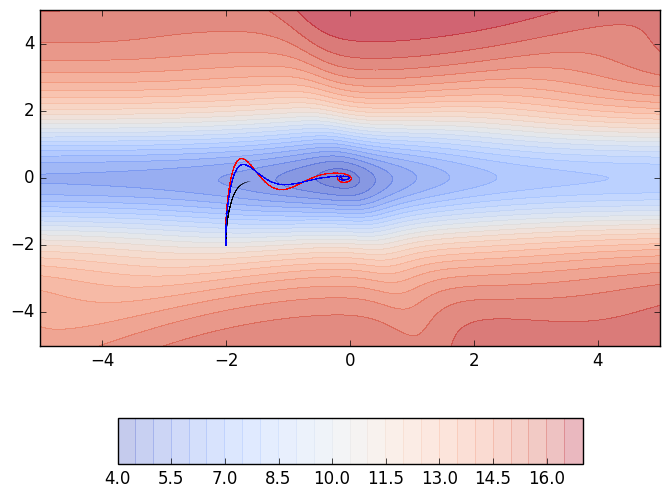
\includegraphics[scale=0.3]{images/module9/nag7/2d_path50.png}}% get width and height
					\node[above right,inner sep=0pt] at (0,0)  {\usebox{0}};
					\node[red,font=\small](w) at (0.5\wd0,0.23\ht0) {w};
					\node[red,font=\small](b) at (0,0.67\ht0) {b};
					\draw[->, line width=0.2mm](w)--(0.6\wd0,0.23\ht0);
					\draw[->, line width=0.2mm](b)--(0,0.8\ht0);
				\end{tikzpicture}
				    
			\end{figure}
			\begin{itemize}\justifying
				\item<9-> Let's see what Adagrad does.... 
			\end{itemize}
			
		\end{overlayarea}
	\end{columns}
\end{frame}

\begin{frame}
	\begin{columns}
		\column{0.6\textwidth}
		\begin{overlayarea}{\textwidth}{\textheight}
			\begin{itemize}\justifying
				\item<34-> By using a parameter specific learning rate it ensures that despite sparsity $w$ gets a higher learning rate and hence larger updates
				\item<35-> Further, it also ensures that if $b$ undergoes a lot of updates its effective learning rate decreases because of the growing denominator
				\item<36-> In practice, this does not work so well if we remove the square root from the denominator \only<37->{(something to ponder about)}
				\item<38-> What's the flipside? \onslide<39->{over time the effective learning rate for $b$ will decay to an extent that there will be no further updates to $b$}
				\item<40-> Can we avoid this?  
			\end{itemize}
		\end{overlayarea}
		
		\column{0.4\textwidth}
		\begin{overlayarea}{\textwidth}{\textheight}
			
			\begin{figure}
				\foreach \n in {0,...,40} {%
					\begin{tikzpicture}
						\sbox0{\includegraphics[scale=0.35]{images/module9/adagrad7/2d_path\n.png}}% get width and height
						\only<\n>{\node[above right,inner sep=0pt] at (0,0)  {\usebox{0}}};
						\only<\n>{\node[red,font=\small](w) at (0.5\wd0,0.23\ht0) {w}};
						\only<\n>{\node[red,font=\small](b) at (0,0.67\ht0) {b}};
						\only<\n>{\draw[->, line width=0.2mm](w)--(0.6\wd0,0.23\ht0)};
						\only<\n>{\draw[->, line width=0.2mm](b)--(0,0.8\ht0)};
					\end{tikzpicture}
				}
			\end{figure}
		\end{overlayarea}
	\end{columns}
\end{frame}


\begin{frame}
	\begin{overlayarea}{\textwidth}{\textheight}
		\vspace{-0.2in}
		\begin{block}{Intuition}
			\begin{itemize}\justifying
				\item<1-> Adagrad decays the learning rate very aggressively (as the denominator grows)
				\item<2-> As a result after a while the frequent parameters will start receiving very small updates because of the decayed learning rate
				\item<3-> To avoid this why not decay the denominator and prevent its rapid growth
			\end{itemize}
		\end{block}
		
		\only<4->{
			\begin{block}{Update rule for RMSProp}
				\begin{align*}
					v_t     & = \beta * v_{t-1} + (1 - \beta) {(\nabla w_{t})}^2            \\
					w_{t+1} & = w_{t} - \frac{\eta}{\sqrt{v_{t} + \epsilon}} * \nabla w_{t} 
					\intertext{... and a similar set of equations for $b_t$}      
				\end{align*}
				
			\end{block}
		}
	\end{overlayarea}
\end{frame}

\begin{frame}
	\begin{columns}
		\column{0.5\textwidth}
		\begin{overlayarea}{\textwidth}{\textheight}
			
			\begin{figure}
				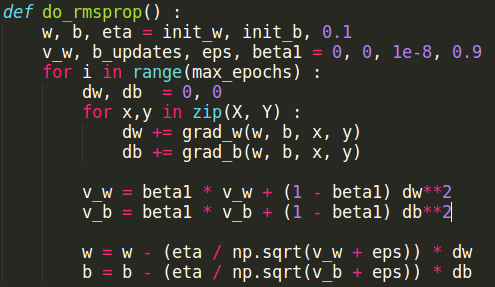
\includegraphics[scale=0.4]{images/module9/pseudo_code_rmsprop_crop.png}
			\end{figure}
			\onslide<29-> {\begin{itemize}\justifying
				\item {Adagrad got stuck when it was close to convergence} \onslide<30-> {(it was no longer able to move in the vertical ($b$) direction because of the decayed learning rate)}
				\end{itemize}}
		\end{overlayarea}
		
		\column{0.5\textwidth}
		\begin{overlayarea}{\textwidth}{\textheight}
			
			\begin{figure}
				\foreach \n in {0,...,29} {%
					\begin{tikzpicture}
						\sbox0{\includegraphics[scale=0.4]{images/module9/rmsprop7/2d_path\n.png}}% get width and height
						\only<\n>{\node[above right,inner sep=0pt] at (0,0)  {\usebox{0}}};
						\only<\n>{\node[red,font=\small](w) at (0.5\wd0,0.23\ht0) {w}};
						\only<\n>{\node[red,font=\small](b) at (0,0.67\ht0) {b}};
						\only<\n>{\draw[->, line width=0.2mm](w)--(0.6\wd0,0.23\ht0)};
						\only<\n>{\draw[->, line width=0.2mm](b)--(0,0.8\ht0)};
					\end{tikzpicture}
				}
				\onslide<30->{
					\begin{tikzpicture}
						\sbox0{\includegraphics[scale=0.4]{images/module9/rmsprop7/2d_path30.png}}% get width and height
						\node[above right,inner sep=0pt] at (0,0)  {\usebox{0}};
						\node[red,font=\small](w) at (0.5\wd0,0.23\ht0) {w};
						\node[red,font=\small](b) at (0,0.67\ht0) {b};
						\draw[->, line width=0.2mm](w)--(0.6\wd0,0.23\ht0);
						\draw[->, line width=0.2mm](b)--(0,0.8\ht0);
					\end{tikzpicture}
				}
				
			\end{figure}
			
			\begin{itemize}\justifying
				\item {\onslide<31> {RMSProp overcomes this problem by being less aggressive on the decay}}
			\end{itemize}
		\end{overlayarea}
	\end{columns}
\end{frame}



\begin{frame}
	\begin{overlayarea}{\textwidth}{\textheight}
		\vspace{-0.2in}
		\begin{block}{Intuition}
			\begin{itemize}\justifying
				\item<1-> Do everything that RMSProp does to solve the decay problem of Adagrad
				\item<2-> Plus use a cumulative history of the gradients
				\item<7-> In practice, $\beta{_1}$ = 0.9 and $\beta{_2}$ = 0.999
			\end{itemize}
		\end{block}
		
		\only<3->{
			\begin{block}{Update rule for Adam}
				\onslide<4-> {
					\begin{align*}
						\onslide<4->{m_t       & = \beta_{1} * m_{t-1} + (1 - \beta_{1}) * \nabla w_{t}              \\}
						\onslide<5->{v_t       & = \beta_{2} * v_{t-1} + (1 - \beta_{2}) * {(\nabla w_{t})}^2        \\}
						\onslide<6->{\hat{m}_t & = \frac{m_t}{1-\beta_1^t}} \hspace{10mm}                            
						\onslide<7->{\hat{v}_t = \frac{v_t}{1-\beta_2^t}}\\
						\onslide<8->{w_{t+1}   & = w_{t} - \frac{\eta}{\sqrt{\hat{v}_{t} + \epsilon}} * \hat{m}_{t}} \\
						\onslide<9-> {         & \text{... and a similar set of equations for $b_t$}}                
					\end{align*}
				}
			\end{block}
		}
	\end{overlayarea}
\end{frame}

\begin{frame}
	\begin{columns}
		\column{0.5\textwidth}
		\begin{overlayarea}{\textwidth}{\textheight}
			
			\begin{figure}
				\includegraphics[scale=0.3]{images/module9/pseudo_code_adam_crop.png}
			\end{figure}
			
			\begin{itemize}\justifying
				\item<25-> As expected, taking a cumulative history gives a speed up  ...
			\end{itemize}
			
		\end{overlayarea}
		
		\column{0.5\textwidth}
		\begin{overlayarea}{\textwidth}{\textheight}
			
			\begin{figure}
				\foreach \n in {0,...,25} {%
					\begin{tikzpicture}
						\sbox0{\includegraphics[scale=0.4]{images/module9/adam7/2d_path\n.png}}% get width and height
						\only<\n>{\node[above right,inner sep=0pt] at (0,0)  {\usebox{0}}};
						\only<\n>{\node[red,font=\small](w) at (0.5\wd0,0.23\ht0) {w}};
						\only<\n>{\node[red,font=\small](b) at (0,0.67\ht0) {b}};
						\only<\n>{\draw[->, line width=0.2mm](w)--(0.6\wd0,0.23\ht0)};
						\only<\n>{\draw[->, line width=0.2mm](b)--(0,0.8\ht0)};
					\end{tikzpicture}
				}
			\end{figure}
		\end{overlayarea}
	\end{columns}
\end{frame}

\begin{frame}
	\begin{overlayarea}{\textwidth}{\textheight}
		\begin{block}{Million dollar question: Which algorithm to use in practice}
			\begin{itemize}\justifying
				\item<1-> Adam seems to be more or less the default choice now ($\beta_1=0.9$, $\beta_2=0.999$ and $\epsilon=1e-8$ )
				\item<2-> Although it is supposed to be robust to initial learning rates, we have observed that for sequence generation problems $\eta = {0.001, 0.0001}$ works best
				\item<3-> Having said that, many papers report that SGD with momentum (Nesterov or classical) with a simple annealing learning rate schedule also works well in practice  (typically, starting with $\eta = {0.001, 0.0001}$ for sequence generation problems) 
				\item<4-> Adam might just be the best choice overall!!
				\item<5-> Some recent work suggest that there is a problem with Adam and it will not converge in some cases
			\end{itemize}
		\end{block}
	\end{overlayarea}
\end{frame}

\begin{frame}
\end{frame}

\begin{frame}
\end{frame}


\end{document}

